\documentclass[../main.tex]{subfiles}

\begin{document}

\section{Methods}
\subsection{Method overview}
\label{sec:methods}
% \subsubsection{Quantum Mechanical methods based on Density Functional Theory (Rana/Hui/Arihant)}
% \begin{itemize}
%     \item Overview of DFT, improvement in XC functionals, VdW corrections and DFT+U/hybrid functionals (Rana 1st draft, Hui 1st review)
    %
    
% Note added MM: Lucy, Chris and I discussed we agreed to shorten the Density Functional Theory section, taking the Hohenberg-Kohn theorem as a given (with references linked), and starting with the Kohn-Sham equations. CS has edited the section. Aim to shorten that part from 5 to 2-3 pages.

\subsubsection{Density Functional Theory (Rana  -- modified by Chris)}
\label{sec:dft}
Density Functional Theory (DFT) is amongst the most accurate methods for atomistic simulations of materials, as it is a first principles quantum mechanical method. This means that it is able to simulate the electrons in materials and how they result in all the observable processes and properties of a  material. As electrons are microscopic particles, to simulate their properties we need to use the theory of quantum mechanics. However, the computational cost of calculations with this theory is very high as all the observable properties are obtained from the wavefunction which is a very complicated function of many variables (proportional to the number of particles we are simulating) and, for exact solution, the computational effort scales (increases) exponentially with the number of particles. Approximate wavefunction-based theories with more favourable computational scaling (such as $\sim N_e^5$ or $\sim N_e^7$ where $N_e$ is the number of electrons in the calculation) have been developed but there also the computational effort is so high that they cannot be applied to molecules with more than a few atoms. 

DFT is a reformulation of quantum electronic structure theory where the central quantity is no longer the wavefunction but the electronic density $\rho(\mathbf{r})$ which is comparatively a much simpler function as the density is a function of only one position variable $\mathbf{r}$. As a result, DFT has lower computational scaling which allows simulations of much larger systems (up to a few hundred atoms on supercomputers). Another advantage of DFT is that it is formally an exact theory. Due to these two significant advantages DFT is today the method of choice for most simulations. 

DFT was originally developed by Hohenberg and Kohn \cite{parr,ph1964B864} and formulated in the form we use it today by Kohn and Sham \cite{wk1965A1133}, so the calculations we perform are often called KS-DFT. In KS-DFT the energy of a material is expressed in the following form:

\begin{equation}
    \label{eq:ks-energy}
    E[\rho] = T_{KS}[\rho] + E_{\rm ext}[\rho] + E_{H}[\rho] + E_{xc}[\rho]
\end{equation}

Where all the terms are expressed as functionals of the density and $T_{KS}[\rho]$ is the kinetic energy of the electrons, $ E_{\rm ext}[\rho]$, is the energy of attraction of the electrons to nuclei (also called external potential energy), $E_{H}[\rho]$, is the classical (Coulomb) electrostatic energy of the electronic density charge distribution (also called Hartree energy) and $E_{xc} $ describes the purely quantum effects of exchange and correlation. 

DFT calculations are performed in an iterative fashion where the density is expressed as a sum of one-electron wavefunctions, $\{ \psi_i \}$, which are called molecular orbitals:

\begin{equation}
    \rho(\mathbf{r}) = \sum_{i=1}^{N_e} | \psi_i(\mathbf{r})|
\end{equation}

and these molecular orbitals are obtained by solving the Kohn-Sham eigenvalue equation:
\begin{equation}
   \left [ -\frac{1}{2}\nabla^2 + \upsilon_{\rm ext}(\mathbf{r}) 
    + \upsilon_{\rm H}[\rho](\mathbf{r}) 
    + \upsilon_{\rm xc}[\rho](\mathbf{r}) \right ]
    = \varepsilon_i \psi_i(\mathbf{r}) 
    \label{eq:ks-evalue-eq}
\end{equation} 
As we can see from the above equation the Hartree, $\upsilon_{\rm H}[\rho]$, and exchange-correlation, $\upsilon_{\rm xc}[\rho]$, potential are functionals of the density, so ultimately they are functionals of the molecular orbitals 
which are the solutions of the equation that we seek. So this equation cannot be solved directly but an iterative procedure called the \emph{self-consistent field (SCF)} process must be followed. The simplest SCF method is to guess a set of $\{ \psi_i \}$ and use them to build and solve (\ref{eq:ks-evalue-eq}) to obtain a new set of $\{ \psi_i \}$ and repeat this process until the $\{ \psi_i \}$ and the energy 
(\ref{eq:ks-energy})
no longer change.

Even though KS-DFT is formally an exact theory it does not provide an explicit expression for the exchange-correlation energy, $E_{\rm xc}[\rho]$. So the exact exchange-correlation functional is unknown or more precisely, unknowable. Thus a very active area of DFT development is to construct approximations of increasing accuracy for $E_{\rm xc}[\rho]$. The simplest approximation is the local density approximation (LDA), where $E_{xc}[\rho(\mathbf{r})]$ is expressed as:

\begin{equation}
    \label{eq:LDA}
    E_{xc}^{LDA}[\rho(\mathbf{r})] = \int\rho(\mathbf{r})\epsilon_{\rm xc}[\rho(\mathbf{r})]\,d\mathbf{r}
\end{equation}

The value of $\epsilon_{\rm xc}$ at some position, $\mathbf{r}$, is computed exclusively from the value of $\rho$ at that position. In practice, $\epsilon_{\rm xc}[\rho(\mathbf{r})]$ describes the exchange and correlation energy per particle of a uniform electron gas of density $\rho$. \cite{Dirac1930}

In general, in a molecular system the electron density is not spatially uniform, even at small volumes of space, which limits the applicability of LDA. More accurate functionals are obtained by the inclusion of a density gradient correction, known as the generalised gradient approximation (GGA) or semi-local functionals. In the GGA, the functionals depend on both the density and the gradient of the density, i.e. $v_{xc}^{\rm GGA} = f(\rho,\nabla\rho)$. Popular examples of GGA functionals are Perdew-Wang GGA (PWGGA) (both exchange and correlation) \cite{PerdewPRB92}, Perdew-Burke-Ernzerhof GGA (PBEGGA), \cite{PBE} and Becke-Lee-Yang-Parr (BLYP), where B stands for the Becke GGA exchange functional \cite{adb19883098} and LYP stands for the Lee-Yang-Parr GGA correlation functional \cite{cl1988785}. Functionals having also contributions from the second derivative of the density are called {\it meta}-GGA functionals. \cite{Perdew-PRL-1999} 

Standard DFT methods fail to describe dispersion effects that are of a non-local electron correlation nature. Consequently, DFT methods are often inaccurate for the investigation of molecular crystals, adsorption on surfaces, and other systems in which dispersion forces due to van der Waals (vdW) gaps between layers play a significant role. Several versions of dispersion corrected DFT (DFT-D) approaches are available, e.g; DFT-D2 \cite{Grimme-1}, DFT-D3 \cite{Grimme-2}, DFT-D4 \cite{Grimme-3}, DFT-D3BJ \cite{Grimme-4,Beke-1}, etc. 

GGA functionals, however, still have problems with self interaction. The hybrid functionals usually offer some improvement over corresponding pure DFT functionals. Of all modern functionals, the B3LYP method is the most popular to date. \cite{adb1993b,cl1988785} It works well for both for structural investigations and for the computation of electronic properties. \cite{Cramer} Another popular hybrid functional, PW1PW, \cite{Bredow00,IslamPRB} was parameterised to reproduce structural, energetic, and electronic properties of solids. A more recent and popular hybrid functional is HSE06, where  the correlation part is defined by a PBE functional and a range-separation approach is used for the exchange part. \cite{HSE06}  

The applicability of the hybrid functionals has large dependence on the type, size, and complexity of the studied systems, as these functionals incur a huge computational cost. Another alternative approach is the DFT+U method, where the effects of strong intra-atomic electronic correlations are modeled by adding an on-site Coulomb repulsion, $U$, and site exchange term, $J$, to the DFT Hamiltonian. \cite{DFT-U-1,DFT-U-2,DFT-U-3} Parameters $U$ and $J$ can be extracted from \textit{ab initio} calculations, but are usually obtained semi-empirically. Inspired by the Hubbard model, the DFT+U method is formulated to improve the ground state description of strongly correlated systems. The Hubbard Hamiltonian describes the strongly correlated electronic states (d and f orbitals), while the rest of the valence electrons are treated by the normal DFT approximations. 

\subsubsection{Linear-Scaling DFT (Arihant -- rewritten by Chris)}
\label{sec:lsdft}
In conventional DFT, solving the Kohn-Sham eigenvalue equations, subject to the required  orthonormality constraint results in a computational cost that scales with the third power 
(it is an  $\mathcal{O}(N^3)$ procedure) with the number of atoms $N$. This is demonstrated in the example of   Figure \ref{fig:ls} which shows the computation time as function of the number of atoms for slabs of graphite of increasing size. This unfavourable scaling is the reason why conventional KS-DFT is  practically unfeasible beyond several hundred atoms. However,  there are many Grand Challenges in materials problems where due to their inherent complexity, in order to build realistic models requires 
thousands of atoms, such as simulations of defects, complex structures of SEI, metallic and semiconductor nanoparticles used in catalysis and battery electrodes, etc.
This need for large-scale DFT calculations has 
 has motivated the development of new theoretical methods which can scale linearly with system size.\cite{Goedecker1999} In these linear-scaling methods,  conventional KS-DFT is reformulated in terms of the one-particle density matrix $\gamma$:

\begin{equation}
    \gamma\left(\rvec,\rprimevec\right)=\sum\limits_i f_i \psi_i\ofrvec\psi_i^*\ofrprimevec   \label{eq:density-matrix-mos}
\end{equation}

which allows us to exploit the   principle of ``nearsightedness of electronic matter'',\cite{Prodans2005} because  the density matrix decays exponentially with the distance $|\rvec-\rprimevec|$ \cite{Prodans2005}, while the molecular orbitals $\{ \psi_\i \}$ are in general fully delocalised over the entire electronic system (molecule, nanoparticle, slab, etc) and do not decay. 
The exponentially-decaying tail of the density matrix can be truncated to develop methods with reduced or linear-scaling computational cost. As the system size (number of atoms) is increased, it reaches a point where the remaining amount of information increases linearly with the size of the system. This can be implemented more efficiently with non-orthogonal localised orbitals $\left\{\ngwf_\alpha\right\}$.\cite{Galli1992, hernandez1995} In this representation, the density matrix can be written as:

\begin{equation}
    \gamma\left(\rvec,\rprimevec\right)=\ngwf_\alpha\ofrvec K^{\alpha\beta} \ngwf_\beta^*\ofrprimevec    
\end{equation}

where the density kernel matrix, $\bf K$ is a generalisation of the MO occupancies $\{ f_i \} $ of equation \ref{eq:density-matrix-mos}, while implicit summation (Einstein convention) is assumed for repeated Greek indices. 

The development of linear-scaling methods has proved a very challenging research topic as the goal of developing methods that accommodate the conflicting requirements of orbital localisation and high accuracy is extremely difficult to achieve. Recent developments towards this goal 
have made this possible by using a dual resolution approach where both the 
$\left\{\ngwf_\alpha\right\}$ and $\bf K$ are optimised self-consistently
during the calculation while being subjected to localisation constraints 
\cite{ONETEP2005}, \cite{Gillan2007}, \cite{Mohr2015}. 
The $\mathcal{O}(N)$ Electronic Total Energy Package (\onetep),\cite{ONETEP2020} is such a code with the unique capability of 
achieving linear-scaling cost while maintaining the near-complete basis 
set accuracy of conventional DFT.  The computational efficiency of this code
is demonstrated on the  graphite example of Figure \ref{fig:ls}, where the linear-scaling behaviour can be clearly seen. As evident,  large DFT  calculations with tens of thousands of atoms can be performed with \onetep. This opens avenues for being able to develop and simulate realistic models of  materials and interfaces in Li-ion batteries.  \onetep{} is being actively developed
and offers a  large and diverse range of capabilities, including different boundary conditions, various exchange–correlation functionals, finite electronic temperature methods for metallic systems, methods for strongly correlated systems, molecular dynamics, vibrational calculations, time-dependent DFT, electronic transport, core loss spectroscopy, implicit solvation, density of states calculations, distributed multipole analysis \cite{ONETEP2020}. 
Recent focus in \onetep{} is on developing into the code electrochemistry tools for battery simulations, aiming to develop  the first atomistic simulation platform (and in particular linear-scaling DFT platform) for electrochemistry. Some of these developments are described in this review in subsection \ref{sec:dft+cont}.

\begin{figure}
    \centering
    \includegraphics[scale=0.5]{figures/linear-scaling-DFT.eps}
    \caption{Comparison of the computational time with the the number of atoms for slabs of graphite of increasing size
     using the \onetep{} linear-scaling DFT code against  a conventional plane wave DFT code. The computations were performed on the Iridis 5 supercomputer at the University of Southampton on $40$ MPI processes with 4 OpenMP threads each (160 cores in total). Reproduced from Ref. \citenum{neutralization-paper}.}
    \label{fig:ls}
\end{figure}

\subsubsection{Nudged Elastic Band} 
\label{sec:methods_neb}

The nudged elastic band (NEB) method is a useful method based on the transition-state theory to find the minimum energy path and the saddle point (or the transition state) between two minimum states (the initial state and the final state).\cite{henkelman2000climbing,henkelman2000improved} The energy difference between the lowest energy state and the saddle point is defined as the activation barrier ($E_a$). 

\begin{figure}
    \centering
    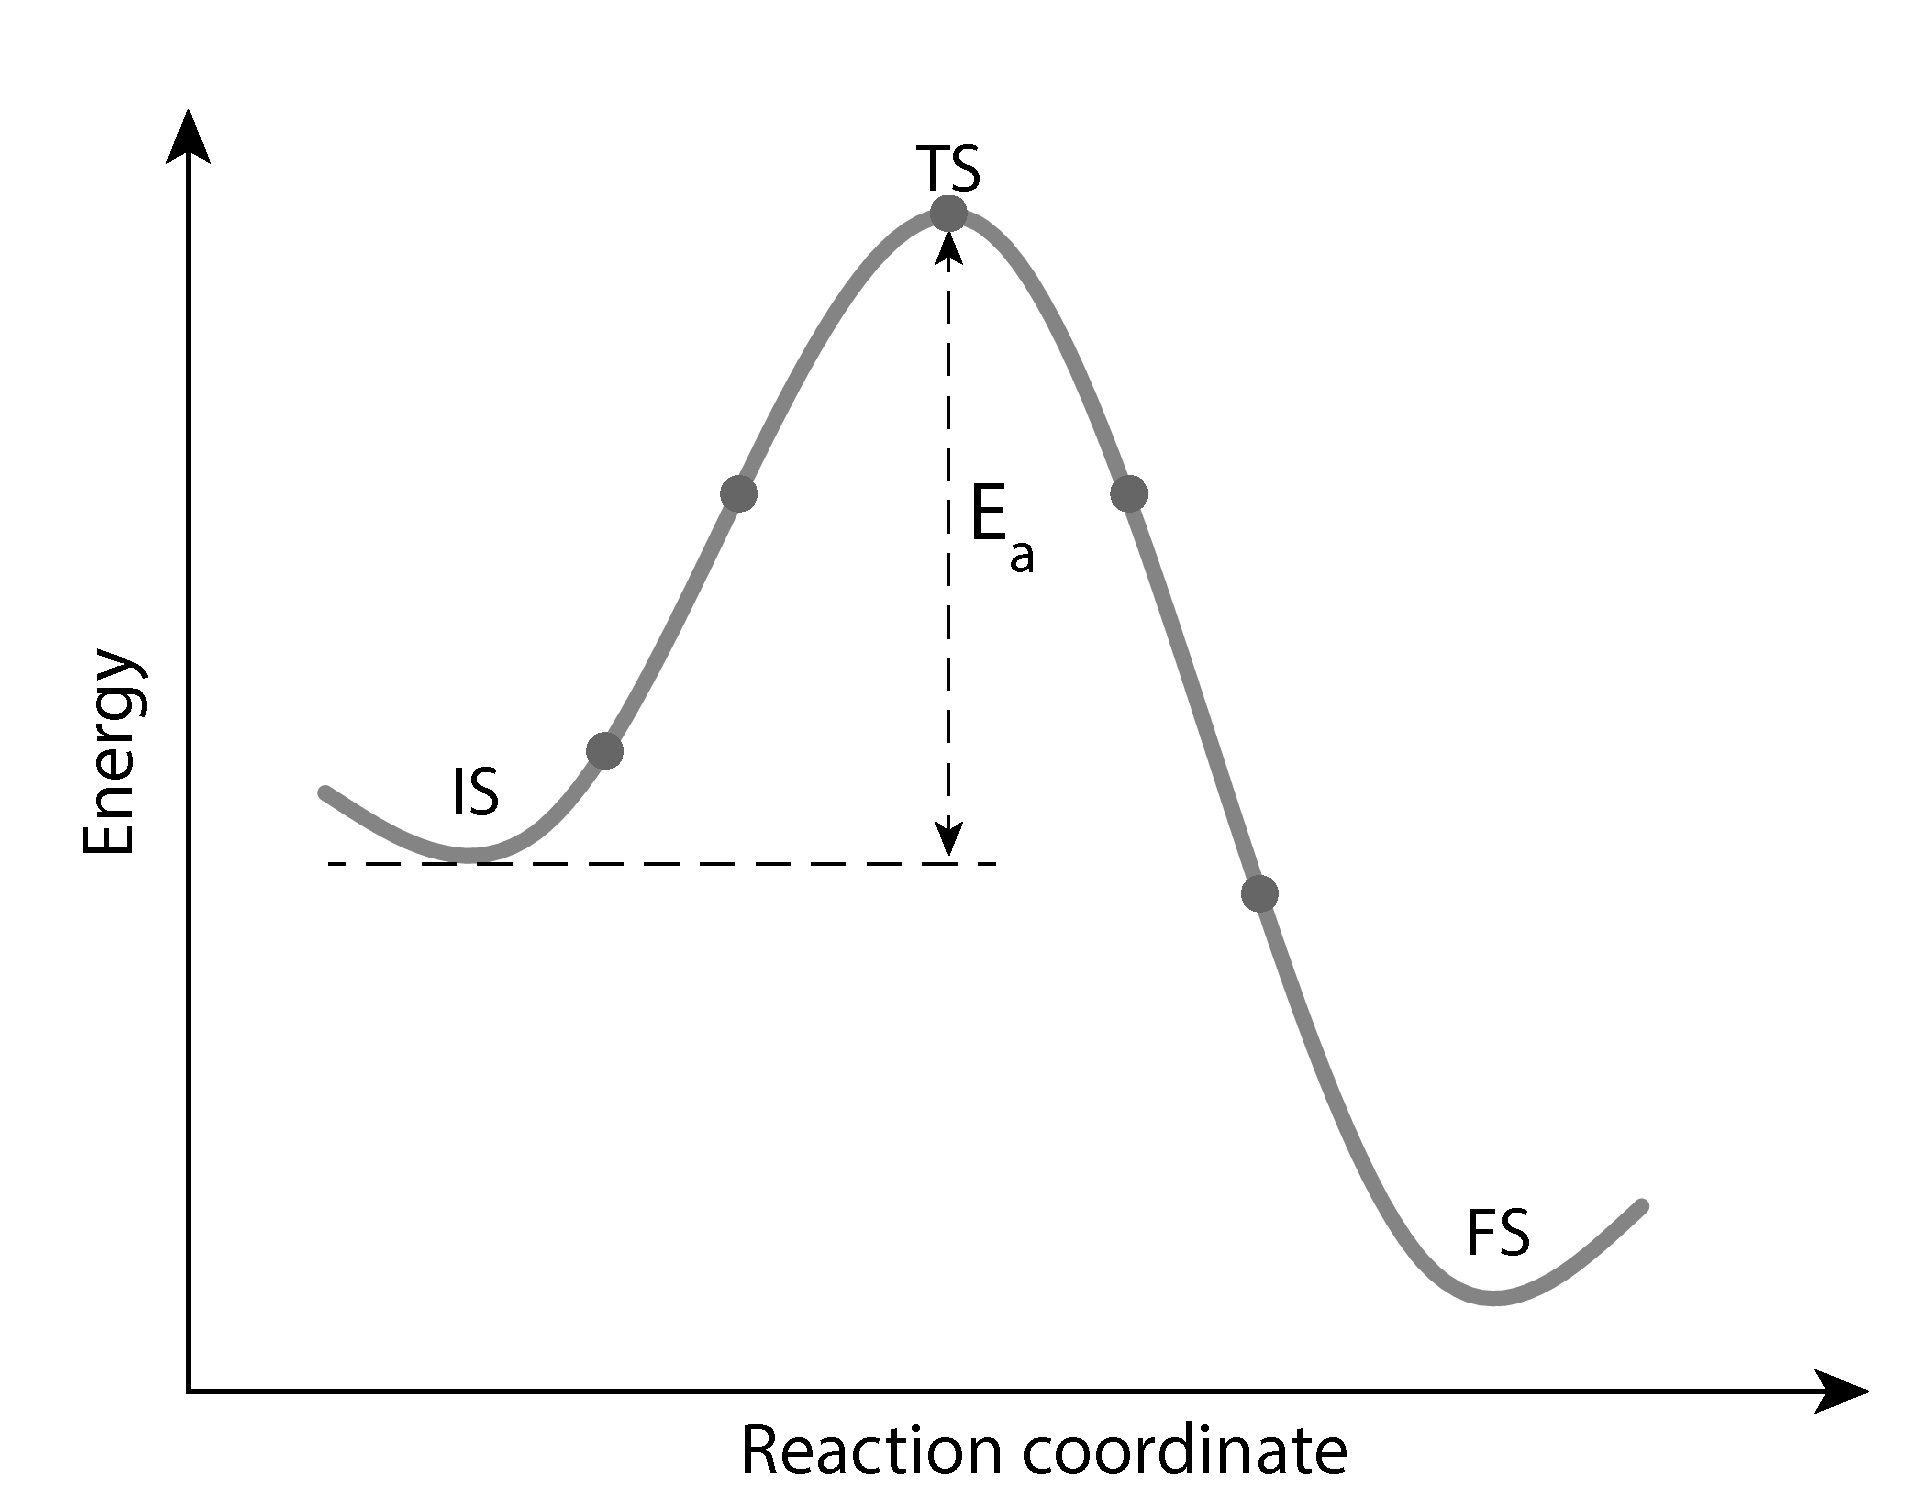
\includegraphics[scale=0.6]{figures/NEB_profile.png}
    \caption{Energy profile of NEB calculation. The IS, TS and FS are the initial state, transition state and final state, respectively. $E_a$ denotes the activation barrier along the reaction path. The grey circles are the images in NEB calculation.}
    \label{fig:NEB_profile}
\end{figure}

The NEB approach initially guesses a number of configurations of several intermediate ``images'' that possibly occur along the reaction coordinate or diffusion path. This set of images can be created by linear interpolation between the initial and final states. The NEB algorithm further conducts constrained optimisation and converges those images along the minimum energy path. Furthermore, fictional spring forces are added between adjacent images to maintain the spacing between adjacent images and the continuity of the reaction or diffusion path. The NEB approach is widely applied in the various studies such as chemical reaction search in catalytic systems or ion diffusion in solid materials to determine the energy barriers which can be further put into the framework of kinetic model.\cite{peng2020lithium,Mercer2021}



\subsubsection{Cluster expansion (Chao)}
\label{sec:cluster_expansion}
The cluster expansion method is a statistical approach to sample the phase space at finite temperature.\cite{sanchez1984generalized,de1994cluster,blum2004mixed} This method aims to investigate the mixing of two or more atoms for a given lattice symmetry by changing the concentration of different atom types and efficiently computing the energy, typically with the accuracy of performing a DFT calculation. Here, if we replace some atoms of a given species with another species, we can take the approach from the Ising model \cite{gallavotti2013statistical} where each lattice site is assigned as a spin variable to simulate the magnetic properties.\cite{persson2010} For example, for a binary alloy system including atom A and B, the occupation of each site can be described by a spin-like variable, i.e $\sigma_i$= +1 if the site is occupied by atom A, and $\sigma_i$= -1 if the site is occupied by atom B, as shown in Figure~\ref{fig:cluster}. The configuration can then be written as $\sigma$=( $\sigma_1$, …, $\sigma_n$). Accordingly, the energy of each configuration can be expressed as: $E\equiv E$($\sigma_1$,…,$\sigma_n$).

\begin{figure}
    \centering
    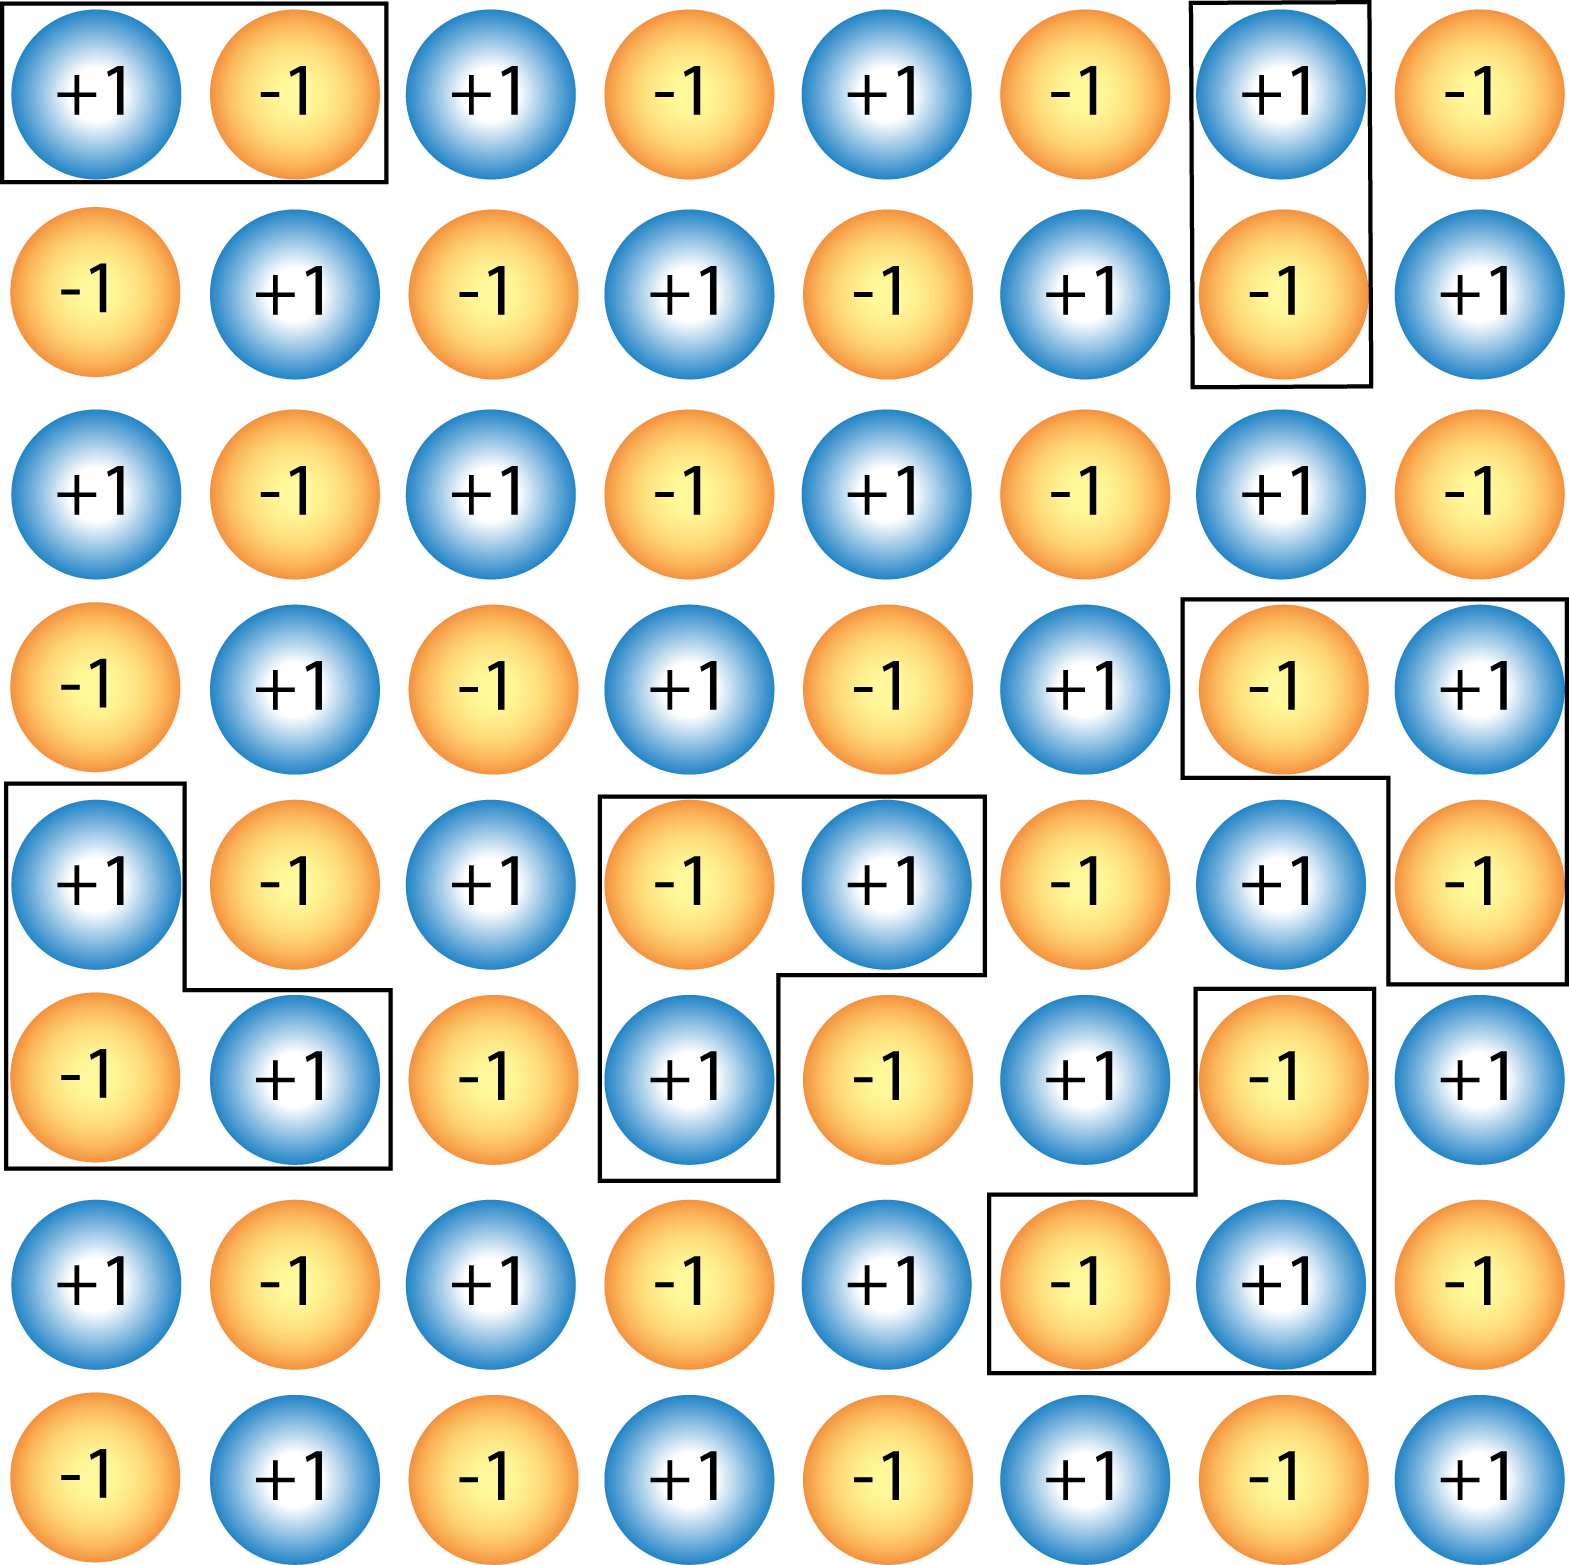
\includegraphics[scale=0.5]{figures/clusters.png}
    \caption{A 2D (8$\times$8) structure including several clusters. +1 and -1 are the lattice sites assigned with different spins.}
    \label{fig:cluster}
\end{figure}

To compute the E($\sigma$), generally all the possible configurations should be sampled. A set of interactions should be considered such as nearest neighbouring pair interaction, second nearest neighbouring pair interaction, triplet interaction, quadruplet interaction, and up to many body interactions (Figure~\ref{fig:cluster}). The combination of those interactions can be ascribed to different ``clusters ($\alpha$)''. Including all the cluster interactions, the energy can be expressed as:

\begin{equation}
    \centering
    {E}_{\alpha}=\sum_\alpha {m_\alpha}{J_\alpha}{\bar{\Pi}_\alpha(\sigma)}
    \label{eq:clusters}
\end{equation} 

where $m_\alpha$ is the multiplicity of the cluster $\alpha$ that can be obtained by considering all the point symmetries in the lattice cell; $J_\alpha$ is the effective cluster interaction (ECI) associated with a cluster $\alpha$; $\bar{\Pi}_\alpha(\sigma)$ is the correlation matrix of normalised spin-products for a particular cluster of the entire lattice and can be obtained via:

\begin{equation}
    \centering
    {\bar{\Pi}_\alpha(\sigma)}=\frac{1}{N{m_\alpha}}\sum_{i\in\alpha} {\Pi{\sigma_i}}
    \label{eq:correlation_matrix}
\end{equation} 

where N is the number of parent lattice cells required to generate the configuration $\sigma$. Theoretically, the expansion should screen over all possible clusters, however, it is not practical to predict the energy as a certain number of clusters might reach the accuracy we need for the calculations. The point symmetries of the lattice should also be applied and we can nominate the clusters the same ECI for those belonging to the equivalent space group.\cite{van2001first} A reduced number of first-principles calculations are  therefore required. Accordingly, $\Pi_\alpha(\sigma)$ can be truncated after a polynomial corresponding to some maximal sized clusters and the coefficient $J_\alpha$ can be deduced from first-principles calculations. If we calculate the energy of an A-B alloy system and consider only four clusters, the cluster expansion matrix can be expressed as:

\begin{equation}
{\left( \begin{array}{cccc}
{E_1}\\
{E_2}\\
{E_3}\\
{E_4}
\end{array}\right)}=
{\left( \begin{array}{cccc}
{\Pi_1}(1) & {\Pi_2}(1) & {\Pi_3}(1) & {\Pi_4}(1) \\
{\Pi_1}(2) & {\Pi_2}(2) & {\Pi_3}(2) & {\Pi_4}(2)  \\
{\Pi_1}(3) & {\Pi_2}(3) & {\Pi_3}(3) & {\Pi_4}(3)  \\
{\Pi_1}(4) & {\Pi_2}(4) & {\Pi_3}(4) & {\Pi_4}(4) 
\end{array}\right)}
{\left(\begin{array}{cccc}
{J_1}\\
{J_2}\\
{J_3}\\
{J_4}
\end{array}\right)}
\end{equation}

The effective interaction coefficient $J_\alpha$ can be obtained via inverting the matrix above by using the energies from first-principles calculations. 

Various codes exist to link the results of first-principles calculations with cluster expansion codes, such as the Alloy Theoretic Automated Toolkit (AT-AT) \cite{avdw:atat2,avdw:atat,avdw:maps},  A Clusters Approach to Statistical Mechanics (CASM) \cite{natarajan2017} or the \textit{ab initio} random structure search (AIRSS) \cite{Pickard_2011}.


\subsubsection{Lattice gas and Monte Carlo (Mike)}
\label{sec:monte_carlo}

Lattice gas methods simulate the system state as an array of points \cite{Binder2009book}. This data structure is ideally suited to represent periodic, crystalline systems, but extensions to more complex systems are possible. In atomistic simulations, the array values denote the occupation of particular sites by certain types of atoms. The evolution of the system state can then be computed in terms of changes in those array values, i.e. site occupancies \cite{Binder2009book}.
    
In the Ising Hamiltonian described in the previous section, each site can be in either a +1 or -1 state \cite{lee1952}. This data structure is suited to studying the thermodynamics and kinetics of binary alloys \cite{PMERCER2016394,oviedo2015underpotential}. Simplistically, a lithium ion battery intercalation material can be represented as a binary alloy of lithium atoms and vacancies within an Ising model \cite{persson2010,mercer_influence_2017,Kim2001ThermodynamicAK}, as applied in the specific examples in the subsequent sections.  
    
The interaction Hamiltonian describes how the energy of the system depends on the configuration of the lattice. For a simple interaction model, it is possible to perform a direct evaluation of the partition function, $Z$, via:
    
\begin{equation}
        Z = \sum_{i}e^{-\beta E_{i}},
        \label{eq:partition_fn}
\end{equation}

where $E_{i}$ is the energy of state $i$, and $\beta = 1/kT$ ($k =$ Boltzmann constant; $T=$ absolute temperature). Once $Z$ is known, the rest of the thermodynamic properties of the system can easily be determined \cite{Mercer2019,Leiva2017b,schlueter_quantifying_2018}. In a two level system \cite{Leiva2017b}, the number of states in equation~\ref{eq:partition_fn} can be reduced to scale linearly with the number of particles in the system, making the summation computationally tractable \cite{Mercer2019,Leiva2017b,schlueter_quantifying_2018}. Measurable quantities, like the open circuit voltage (OCV), voltammograms, and partial molar enthalpy and entropy can be simulated \cite{schlueter_quantifying_2018,Leiva2017b,Mercer2019}. This approach has been applied to lithium intercalation in lithium manganese oxide (LMO) \cite{schlueter_quantifying_2018} and graphite \cite{Mercer2019,Leiva2017b}, as demonstrated in section~\ref{sec:anodes_entropy}. The interactions between the particles can be approximated by taking the average occupation in two levels, allowing ordered structures like graphite stages to be modelled. This approach represents a step in complexity beyond the assumption of simple solid solution behaviour, which is still commonly applied in continuum level models. \citeauthor{HAFTBARADARAN2011361} The approach is closely related to the phase field models applied by \citeauthor{Bazant2017} to systems such as lithium iron phosphate (LFP) and graphite \cite{Bazant2017,guo2016,peng2011}.

For a more general and realistic interaction Hamiltonian, there are too many energy states for the direct determination of equation~\ref{eq:partition_fn} for an analytical determination of the thermodynamics to be feasible. In that case, Monte Carlo methods are useful for calculating thermodynamic properties. This is true for the Ising model defined in section~\ref{sec:cluster_expansion} when represented in more than one dimension, as is the case in most practical systems.  It is then more practical to obtain the thermodynamic properties by the Metropolis algorithm \cite{Metropolis1953}. Following the Markov chain of states, the limiting distribution equals the probability distribution of the thermodynamic ensemble. Properties of interest can be obtained from taking the average of sampled configurations once the distribution has reached equilibrium \cite{oviedo2015underpotential}.

Inputting a chemical potential, $\mu$, in the grand canonical ensemble, the ground state properties of the system are obtained as follows. For a lithium ion battery, $\mu$ represents the chemical potential of intercalated Li in the host, i.e. the electrode potential, described in section~\ref{sec:properties_equilibriumvoltage}. Computing the average occupation, $\langle N \rangle$, of particles in the system at each $\mu$ value, therefore allows the equilibrium potential to be simulated at any input temperature, $T$. Along with $\langle N \rangle$, the average internal energy $\langle{E}\rangle>$ is a useful parameter to check the convergence of the simulation results with respect to the system size \cite{mercer_influence_2017,Binder2009book,Kim2001ThermodynamicAK,darling1999}.

Variances can be computed to check the system size convergence and derive experimentally measurable parameters. For example, the configurational component of the heat capacity at constant volume, $C_{V}$, given by:

\begin{equation}
    C_{V} = \frac{\beta}{T}\left(\langle{E^{2}}\rangle -{\langle{E}\rangle}^{2}\right) =  \frac{\beta}{T}\rm{var}(E),
    \label{eq:mc_heat_cap}
\end{equation}

where $\rm{var}($E$)$ is the variance of $E$. The vibrational and electronic components of $C_{V}$ must be determined by other means, such as the approaches outlined in section~\ref{sec:thermal_electronic_vibrational}. 

It is also possible to determine voltammograms from $\rm{var}(N)$, as explained in refs. \cite{mercer_influence_2017,darling1999}. If the covariance of $U$ and $N$ is also known, the partial molar internal energy, $\partial{U}/\partial{N}$ and partial molar entropy $\partial{S}/\partial{N}$ can be obtained, as defined elsewhere \cite{mercer_influence_2017,Kim2001ThermodynamicAK}. These parameters can be compared with experimental parameters from ``entropy profiling'' or calorimetry \cite{mercer_influence_2017,schlueter_quantifying_2018,Mercer2019,THOMAS2003844} and input into a dynamic models such as kinetic Monte Carlo (kMC) \cite{gavilan-arriazu_kinetic_2020,darling1999,gavilan-arriazu_effect_2020,persson2010}, or Molecular Dynamics (MD) to describe temperature dependent behaviour. A dedicated review of kMC is forthcoming; however, the technique is briefly described by \citeauthor{VanderVen2020}. \cite{VanderVen2020} MD is described in the following section.

\subsubsection{Molecular Dynamics (Lucy/Julian)}
\label{sec:molecular_dynamics}
Molecular Dynamics (MD) is an approach which probes the dynamic evolution of a system over time. The crucial input for these simulations is the potential energy surface, PES, which describes the interactions between atoms. In \textit{ab initio} MD (AIMD), this is described by solving the Schr\"{o}dinger equation, whereas in a classical mechanics framework the interactions are described using parameterised interatomic potentials.

There are multiple forms interatomic potentials can take, with their relevancy and accuracy relating to the system and study being conducted. Atoms are either attracted or repelled by one another based on their interatomic distance, $r$, to reduce their potential energy to a minimum, $r_{eq}$. This is known as a pair-interaction, which can be used to calculate the force, $\overrightarrow{\rm F}$ acting on each atom as given by:

\begin{equation}
    \overrightarrow{\rm F_i} = \sum_j {\overrightarrow{\nabla}}E(r_{ij})
\end{equation}

In complex systems there is a ``net effect'' of the $N$ surrounding atoms which can be accounted for by calculating the vector summation of each pair-interaction contribution. Within ionic materials the pair interactions are dominant and therefore it is computationally tractable to truncate the expression after the first term \cite{harding_computer_1990} to give an approximation of the pair potential. The charged nature of ions form a coulombic interaction, where the relatively slow decay of $\frac{1}{r}$ as $r$ increases, giving rise to the long range component of the potential. The general term for the total potential can therefore be written as:

\begin{equation}
    E(r_{ij}) = \frac{Q_i Q_j}{4\pi \varepsilon_0 r_{ij}} + \Phi_{sr}
\end{equation}

Where $i$ and $j$ are ions of charge $Q_i$ and $Q_j$ at a distance of $r_{ij}$, and $\varepsilon_0$ is the permittivity of free space. $\Phi_{sr}$ is used to denote the remaining short-range interactions.

For ionic solids, including cathode materials, a common choice for an interatomic potential is a Coulomb-Buckingham potential \cite{buckingham_classical_1938}, derived from the Born model of the ionic solid \cite{born_1932, mayer_1932}, where the potential energy of the system can be expressed as:

\begin{equation}
    E(r_{ij}) =  \sum_{ij} \frac{Q_i Q_j}{4\pi \varepsilon_0 r_{ij}} + \sum_{ij} A \ exp(\frac{-r_{ij}}{\rho}) - Cr_{ij}^{-6}
    \label{eqn:buckingham}
\end{equation}

Here, $A$, $\rho$, and $C$ are constants.

Molecular dynamics simulations can be performed using a range of ensembles, with the most commonly used being microcanonical (NVE), canonical (NVT), and isothermal-isobaric (NPT) ensembles. \cite{todorov2006dl_poly_3, PLIMPTON19951, gale_gulp_1997} Here, the number of atoms (N), volume (V), energy (E), temperature (T), and pressure (P) are conserved within the respective ensembles. Within the NVT and NPT ensembles the energy of endothermic and exothermic processes is exchanged with a thermostat. A variety of thermostat algorithms are available, with some of the most popular methods including the Nos\'{e}-Hoover, Berendsen, and Andersen thermostats. \cite{todorov2006dl_poly_3, PLIMPTON19951, gale_gulp_1997} For NPT ensembles, a barostat is also applied to control pressure.

Ab-initio Molecular dynamics (AIMD) is able to capture events that classical MD cannot, including bond breaking, and bond formation. AIMD also assumes that the dynamics of particles can be treated classically and that the equation of motion for all particles can be written as 
\begin{gather}\label{eq:eom}
    M_I\"{\textbf{R}}_I=-\nabla_I\left[ \varepsilon_0(\textbf{R})+V_{NN}(\textbf{R})\right]
\end{gather}
where $\textbf{R}$ denotes all nuclear coordinates, $\varepsilon_0(\textbf{R}$ represents the ground state energy of the system at that given nuclear configuration, and $V_{NN}(\textbf{R}$ represents the nuclear-nuclear coulomb repulsion at that given nuclear configuration. 
Most modern techniques achieve this feat by solving the schr\"{o}dinger equation using Kohn-Sham DFT (see sec. \ref{sec:dft}). AIMD can be broadly split up into two main categories, Born-Oppenheimer dynamics and Car-Parrinello extended Langragian. The Born-Oppenheimer dynamics method use a sympletic integrator to numerically integrate the equation of motion seen in Eq. \ref{eq:eom}. This is done for each time step. The Car-Perrinello extended Langragian method gives the Kohn-Sham orbitals an artificial time-dependence. To accomplish minimum energy with each new $\textb$ this the orbital dynamics are kept at a temperature different to that of the nuclei.  The new artificial orbitals can then be defined by the Lagragian below

\begin{gather}
    L=\mu \sum_i f_i \int d\textbf{r}|\psi_i(\textbf{r},t)|^2
    +\frac{1}{2}\sum^N_{I=1} M_I\dot{\textbf{R}}^2_I (t)- E\left[{\psi(t)}, \textbf{R}(t)\right]
    +\sum_{i,j} \Lambda_{ij}\left[\int d\textbf{r}\psi^*_{\,i}(\textbf{r},t)\psi_j(\textbf{r}, t)- \delta_{ij}\right]
\end{gather}

where  $\psi_x(\textbf{r},t)$ are the time dependent kohn-sham orbitals, and $\Lambda_{ij}$ contains a set of of Lagrange multipliers to implement the orthonormality constraint on the orbitals.

The choice between AIMD and classical MD is a trade-off between computational cost, accuracy, and transferability. AIMD is highly accurate, however, it is computationally expensive and scales poorly ($>O(N^3)$), making reachable system sizes and timescales relatively small ($<$1000 atoms, $\sim$100 ps). On the other hand, classical MD is less computationally expensive and can be applied to much larger systems sizes, up to millions of atoms, with longer reachable time scales in the range of nanoseconds. The classical approach however is generally less accurate, as developing an interatomic potential which is sufficiently accurate enough to describe the specific system chemistry is challenging. The development of interatomic potentials is discussed in greater detail in section \ref{sec:potential_fitting}.


\subsection{Method Development}

\subsubsection{Continuum models of electrolyte solutions within Density Functional Theory (Chris Skylaris and Arihant)}
\label{sec:dft+cont}
Electrode-electrolyte interfaces are an important part of Li-ion batteries and a area of active research.\cite{Gauthier2015, Yu2018} The complexity of the structure and formation of electrical double layers at the interface has hindered the understanding of important electrochemical processes. While DFT based electronic structure methods have been successively used to study the solid-state physics in the bulk electrodes of the Li-ion battery, they are inadequate to describe the liquid state, which lacks structural order. This has led to rapid development of methods to describe the electrode-electrolyte interfaces.\cite{Jinnouchi2018} 

The liquid state can be described mainly via explicit solvation,\cite{Hansen2016} implicit solvation,\cite{Sakong2015} or both.\cite{Skyner2015} In the former, explicit molecules of surrounding solvent and electrolyte are added and considered on an equal footing as the electrode. The surrounding electrolyte molecules not only neutralise the surface charge but also form bonds and adsorb on the electrode.\cite{Kang2011} More extensive models of electrode-electrolyte interfaces also include an explicit counter-electrode.\cite{Dufils2019, Jorn2013} The addition of a large number of solvent and electrolyte molecules to describe the liquid state drastically increases the configurational degrees of freedom. Sampling this large configurational space leads to an increase in the computational overhead and the loss of focus on the main interface region. While consideration of the first bonding layer of explicit solvent and electrolyte molecules is necessary to describe the local bonding effects and the local effects of the electric field,\cite{Zhang2020} the degrees of freedom of the non-participating solvent and electrolyte molecules far away can be averaged out via an implicit model of the electrolyte solution.\cite{Cramer1999, Tomasi2005} These hybrid quantum-continuum models are based on solving the Poisson-Boltzmann equation (\pbe).\cite{Grochowski2008} Many DFT+\pbe{} models have been developed recently.\cite{Jinnouchi2008, Gunceler2013, Ringe2016, Nattino2019, Melander2019, Stein2019, DLMG2018, Dziedzic2020, neutralization-paper}

The continuum electrolyte ions with space dependent concentrations $\ci\ofrvec, i=1\dots p$ and charges $\{\zi\}$ create a mobile electrolyte density, $\densmob\ofrvec=\sum\limits_{i=1}^p\zi\ci\ofrvec$. This mobile electrolyte charge density, $\densmob\ofrvec$,  interacts with the quantum charge density, $\dens\ofrvec$, within a mean-field electrostatic potential, $\pot\ofrvec$. This effect can be included in standard DFT by extending the standard free energy functional to include the mean-field electrostatic potential $\pot\ofrvec$ and the mobile charge concentrations, $\ci\ofrvec$, as:\cite{Dziedzic2020}

\begin{equation}
    E\left[\dens\ofrvec\right]\rightarrow \Omega\left[\dens\ofrvec,\pot\ofrvec,\ci\ofrvec\right]
\end{equation}

The variation of the free energy functional with the electrostatic potential, $\pot\ofrvec$, gives the Poisson-Boltzmann equation \pbe{}.

\begin{equation}
    \label{eq:pbe}
    \nabla\cdot\left[\veps\ofrvec\nabla\nu\ofrvec\right]=-4\pi\left[\dens\ofrvec+\densmob\ofrvec\right]
\end{equation}

The \pbe{} not only includes the quantum charge density, $\dens\ofrvec$, as in standard DFT calculation in vacuum, but also the effect of solvent in terms of a continuum dielectric with permittivity function, $\veps\ofrvec$, and mobile charge density of electrolyte ions, $\densmob\ofrvec$. The permittivity function is chosen as a smooth function with value varying from 1 in the quantum region to $\veps^\infty$ in the solvent region:\cite{Nattino2019}

\begin{equation}
    \veps\ofrvec=1+\left(\veps^\infty-1\right)s\ofrvec
\end{equation}

where $s\ofrvec$ is a smooth interface function varying from 0 in the quantum region to 1 in the solvent. Several choices for the interface function have been discussed in Ref. \citenum{Andreussi2012}. The variation of the free energy functional with ion concentrations, $\ci\ofrvec$, gives the Boltzmann expression for ionic concentrations:

\begin{equation}
    \label{eq:cig}
    \ci\ofrvec = \cif\lambda(\rvec) \exp \left(-\frac{z_i\pot(\rvec)}{\kb T} +\frac{\muexi}{\kb T} \right), \ i=1\dots{}p
\end{equation}

where $\{\cif\}$ and $\{\muexi\}$ are the bulk concentrations and excess chemical potentials of the electrolyte ions. The mobile charge density of electrolyte ions $\densmob\ofrvec=\sum\limits_{i=1}^p\zi\ci\ofrvec$ is shown schematically in Fig. \ref{fig:DFT+continuum}. As the interaction with mobile electrolyte charge is purely electrostatic and excludes any quantum effects such as Pauli repulsion, there is a problem of electrolyte charge getting accumulated infinitely close to the electrode. In order to prevent the problem of charge accumulation near the boundary of the quantum solute, the models include an electrolyte accessibility function, $\acc\ofrvec$, which varies from 0 near the electrode to 1 in the bulk electrolyte region.\cite{Fisicaro2017, Sundararaman2018, Stein2019} One of the ways of defining such an accessibility function is as a product of atom-centered interlocking spheres of error functions:\cite{Dziedzic2020}

\begin{figure}
    \centering
    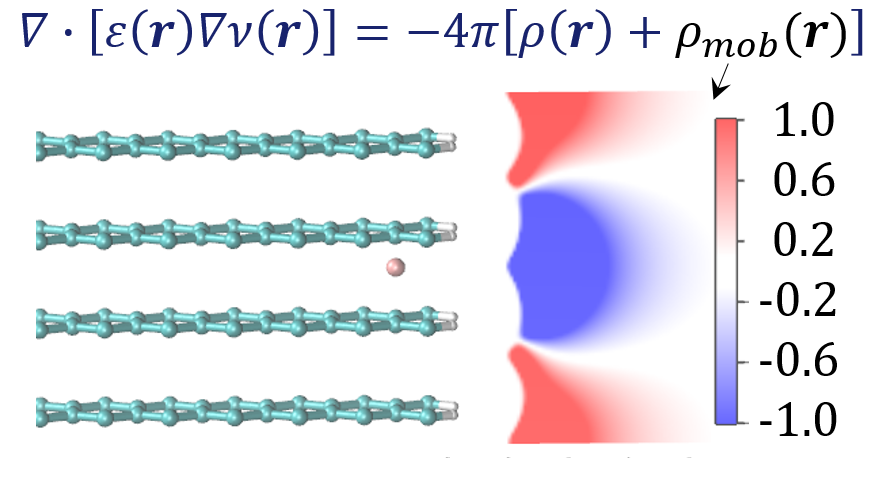
\includegraphics[scale=0.7]{figures/DFT+Continuum.png}
    \caption{DFT simulation of a Lithiated graphite interface in contact with an implicit electrolyte solution based on the solution of Poisson-Boltzmann equation. Reproduced from Ref. \citenum{Dziedzic2020}}
    \label{fig:DFT+continuum}
\end{figure}

\begin{equation}
    \label{eq:access}
    %\nonumber
    \acc\ofrvec = \prod\limits_{k}^{n_\textrm{atoms}}\half  \left[1+\textrm{erf}\left(\frac{|\textbf{r}-\textbf{R}_k|-R^{\rm solute}_k(\denselec^\acc)-R^{\rm solvent}_k}{\sigma}\right)\right],
\end{equation}

where $\sigma$ is a smearing width $(0<\sigma<0.5~a_0)$. This description of the radius of interlocking spheres derives from a physical picture: the electrolyte ions are restricted from the quantum electrode up to a distance that incorporates not only the solute size but also a solvation shell radius. The solute size is described in terms of an isoradius of electronic density, $\denselec^\acc$. The solvation shell radius, $R^{\rm solvent}_k$, which depends on the solvent, is added to the solute size to calculate the overall radius of interlocking spheres for the accessibility function.

The electrostatic potential, $\pot\ofrvec$ obtained from eq. \ref{eq:pbe} is due to the entire electrode-electrolyte interface, where the electrode is treated quantum mechanically and the electrolyte solution as a continuum. Variation of the free energy functional with electronic density gives the Kohn-Sham equations in the total electrostatic potential with additional terms for the variation of interface function with electronic density.\cite{Dziedzic2011, Ringe2016} Solvation energies are defined as:\cite{Ringe2016, Stein2019}

\begin{align}
    \Delta\Omega &=\Omega-\Omega_{\textrm{vac}}-\Omega_{\textrm{electrolyte}} \\
    &=\Omega\left[\dens\ofrvec,\{\ci\ofrvec\},\pot\ofrvec\right] \\
    \nonumber
    &-\Omega\left[\dens_{\textrm{vac}}\ofrvec,\{\ci\ofrvec\}=0,\pot_{\textrm{vac}}\ofrvec\right] \\
    \nonumber
    &-\Omega\left[\dens\ofrvec=0,\{\ci\ofrvec\}=\{\cif\},\pot\ofrvec=0\right]
    \nonumber,
\end{align}

where the respective terms can be computed as the total free energy in the electrolyte solution, the total free energy in vacuum, and the total free energy of the pure electrolyte.\cite{Dziedzic2020} The electrolyte effect on solvation energies can be computed as the difference of solvation energy in electrolyte at $\{\cif\}$ and solvation energy in pure solvent at $\{\cif=0\}$:

\begin{align}
    \Delta\Delta\Omega    &= \Delta\Omega\left[{\{\cif\}}\right]-\Delta\Omega\left[{\{\cif=0\}}\right] \\
    &= \Omega - \Omega_{\textrm{sol}} - \Omega_{\textrm{electrolyte}},
\end{align}

where the respective terms are computed as the total free energy in the electrolyte solution, $\{\cif\}$, the total free energy in pure solvent, $\{\cif=0\}$, and the total free energy of the pure electrolyte. 



\subsubsection{Extracting Stefan-Maxwell diffusivities from MD, and Onsager-Casimir decay of fluctuations hypothesis (MZ)}
\label{sec:stefan-maxwell}
%v2, Jan 30, 2021
The Onsager decay of fluctuation hypothesis dictates that the autocorrelation functions of fluctuating quantities, in the linearised approximation, satisfy the same equations that the linearisation of the continuum transport equations provides. Such theory has been developed by Monroe, Wheeler and Newman
\cite{mwn2006,mwn2009,mwn2015} .

In continuum theory, material balance equations for species molar concentrations, $c_i$, are given by

\begin{equation} \begin{array}{l}
    \displaystyle \frac{\partial c_i}{\partial t} = - \nabla \mathbf{J}_i  ,
    \\
    \mathbf{J}_i  = c_i \mathbf{v}_i ,
    \label{massbalance}
\end{array} \end{equation}
\noindent where $\mathbf{v}_i$ are velocities of species $i$. The thermodynamic equation of state at a constant pressure implies a relation among molar concentrations, $c_i$:

\begin{equation}
    \displaystyle\sum_{i=1}^n c_i \bar{V}_i ( \, \mathbf{y} ) \, =1,
\end{equation}

\noindent where $\mathbf{y} = (y_1, y_2, \ldots y_n)$ are molar fractions,  $y_j = \frac{c_j}{c_T}$ , $\bar{V}_i$ are partial volumes, $\bar{V}_i = \left. \left(\, \displaystyle\frac{\partial V}{\partial n_i} \right)\, \right\vert_{P,T, n_j,j\neq i}$,  and $c_T = \sum_j c_j$ is the total concentration.

\begin{equation}
    \displaystyle \frac{1}{c_T} = \displaystyle\sum_{i=1}^n y_i \bar{V}_i ( \, \mathbf{y} ) .
    \label{cT}
\end{equation}

From the general principles of nonequilibrium thermodynamics, there is a relationship between generalized forces and fluxes. For systems which are locally near equilibrium at constant temperature and pressure, this implies a Stefan-Maxwell relationship between the gradients of the chemical potentials (``forces'')  and the fluxes:
%cite Neuman and Goyal

\begin{equation} \begin{array}{l}
    \displaystyle c_i \nabla \mu_i = \displaystyle \sum_{j\neq i}  K_{ij} (\mathbf{v}_j - \mathbf{v}_i), \
    K_{ij}= R  T  \frac{c_i c_j }{c_T D_{ij}}.
    \label{StM:K}
\end{array} \end{equation}

\noindent where $D_{ij}= D_{ji},$ $i \neq j,$ are the relative diffusion coefficients of species $i$ and $j$. ~\ref{StM:K}  ensures that the entropy production rate $g_s$ is non-negative:

\begin{equation}
    T g_s = - \sum_{i=1}^n c_i \nabla \mu_i ( \, \mathbf{v}_i - \mathbf{v}_{\mbox{ref}} ) = \frac{R  T}{2} \displaystyle\sum_{ij=1}  \frac{c_i c_j}{c_T D_{ij}} ( \, \mathbf{v}_i -\mathbf{v}_j ) \,^2 \geq 0 ,
    \label{gs}
\end{equation}

\noindent where $\mathbf{v}_{\mbox{ref}}$ is a reference velocity, which does not affect $g_s$ due to the Gibbs-Duhem relations ~\ref{GibbsDu}.

%The ``self-diffusion'' coefficient, where $i=j$, does not appear in this approach to continuum modeling. To link this approach to other approaches one may consider a single particle as a separate species \cite{2002PhDWheeler}.

%It is important to note that
To find fluxes $\mathbf{J}$ in ~\ref{massbalance} we need to know the species velocities. However, we {\bf cannot} just invert Stefan-Maxwell relations ~\ref{StM:K} to find all those velocities, as adding
%the same
a reference velocity to all the species velocities does not change the right hand side of ~\ref{StM:K}.
Indeed, ~\ref{StM:K} can be written as a linear system
\begin{equation} \begin{array}{l}
    \displaystyle \sum_{j }  M_{ij}  \mathbf{v}_j  = c_i \nabla \mu_i , \
    M_{ij}= \left\{  \begin{array}{rl}  K_{ij} & i\neq j \\ -  \displaystyle \sum_{k\neq i} K_{ik} & i = j\end{array} \right. ,
    \label{StM:M}
\end{array} \end{equation}
\noindent where $K_{ij}$ is defined in ~\ref{StM:K}. The matrix $M = \left\{ M_{ij} \right\}$ is a symmetric matrix with zero margins for all rows or columns,
$$
M= M^T, \  \displaystyle  \sum_{i} M_{ij} = \sum_{j } M_{ij} = 0,
$$

\noindent Such a matrix $M$ is \textbf{not} invertible, as it has a (right and left) nullvector $\mathbf{z}_0= (1,1, \ldots 1)^{T}:$

\begin{equation} \begin{array}{l}
    \displaystyle  \mathbf{z}_0^{T}   \ . \  M = M \ . \ \mathbf{z}_0 = 0.
\end{array} \end{equation}

%Here, the ``self-diffusion'' terms cancel out,

However, due to the Gibbs-Dulem relations, which follow from the thermodynamic identities and extensivity conditions of the Gibbs potential \cite{GoyalMonroe}, the right-hand side of ~\ref{StM:M} is always orthogonal to the nullvector:

\begin{equation}
 \mathbf{z}_0^{T}   \ . \ \left( c  \nabla \mu \right) =   \sum_{i=1}^n c_i \nabla \mu_i = 0.
 \label{GibbsDu}
\end{equation}

Therefore, it follows from the Fredholm alternative in linear algebra that ~\ref{StM:M} can be solved for velocities of the species, up to adding a reference velocity to all the velocities; while such a reference velocity cannot be determined from ~\ref{StM:M}.

Since $\sum_{j } M_{ij} = 0$, we could as well write the velocities relative to velocities of a chosen species. Let's label that species by 0 and consider it to be the solvent:
\begin{equation} \begin{array}{l}
    \displaystyle \sum_{j }  M_{ij} \left(  \mathbf{v}_j - \mathbf{v}_0 \right) = c_i \nabla \mu_i
     \label{StM:MM}
\end{array} \end{equation}
Only $\mathbf{v}_j$ with $j\neq 0$ contribute in the right hand side of equation~\ref{StM:MM}. Also, due to the Gibbs-Duhem relations and since $\sum_{i} M_{ij}=0,$ the equation for $c_0 \nabla \mu_0$ will be automatically satisfied if the remaining equations are. Thus, all the unknowns, $\left(  \mathbf{v}_j - \mathbf{v}_0 \right)$, can be found by considering a reduced system where $i$ in ~\ref{StM:MM} takes only values with $i\neq 0$. We then have the same number of unknowns and equations in such a reduced linear system, and it can be solved.

The diagonal coefficients $M_{ii}$ are nonzero, and by analogy with ~\ref{StM:K}, we introduce the Stefan-Maxwell "self-diffusion" coefficient $D_{ii}$ by
\begin{equation} \begin{array}{l}
    \displaystyle M_{ii} = -\frac{c_i^2 R  T }{c_T D_{ii}},
\end{array} \end{equation}
which yields
\begin{equation} \begin{array}{l}
    \displaystyle  \frac{y_i }{ D_{ii}} = \sum_{k\neq i} \frac{y_k }{ D_{ik}}.
     \label{StM:sd}
\end{array} \end{equation}

In the literature, a version of Stefan-Maxwell relations resolved for the fluxes is also used,
\begin{equation} \begin{array}{l}
    \displaystyle y_i \mathbf{v}_i  = - \frac{1}{RT} \sum_{j} L_{ij} \nabla \mu_j .
    \label{StM:L}
\end{array} \end{equation}
\noindent In view of the above, extra care is needed in using the pseudo-inverse form ~\ref{StM:L}, since gradients of chemical potentials are not all independent and must satisfy the Gibbs-Duhem relations, while species velocities are determined by such gradients only up to a reference velocity.

To relate continuum models with molecular dynamics, we need a linearized version of the continuum modeling equations. We need to remember that only $(n-1)$  molar fractions $\left\{ y_i \right\}$ are linearly independent, since $\sum_{i=1}^{n} y_i =1.$ Thus we can express  one of the y, e.g. $y_n,$ in terms of all the other $y$:

\begin{equation}
    y_n = - \displaystyle\sum_{i=1}^{n-1} y_i.
\end{equation}

We linearize the equations by expanding those to the first order about the thermodynamic equilibrium values, denoted by $\infty$  ($y_i^\infty$ are constants determined by composition, and $\mathbf{v}_i^{\infty} = 0$):

\begin{equation} \begin{array}{l}
    y_i = y_i^\infty + y_i^{(1)}+ \ldots, i=1,2\ldots n-1, \quad y_n = - \displaystyle\sum_{i=1}^{n-1} y_i,
    \\
    \mathbf{v}_i = 0 + \mathbf{v}_i^{(1)} + \ldots .
\end{array} \end{equation}

\noindent Linearization of the Stefan-Maxwell equations yields:

\begin{equation} \begin{array}{l}
    \nabla \mu_i^{(1)} = RT \displaystyle \sum_{j=1}^{n} \frac{y_j^{\infty}}{D_{ij}^{\infty}} ( \, \mathbf{v}_j^{(1)} - \mathbf{v}_i^{(1)}) \, , i =1,2,\ldots n-1,
    \\
    \nabla \mu_i^{(1)} = \displaystyle \frac{RT}{y_i^{\infty}}\sum_{j=1}^{n-1} Q_{ij} \nabla  y_j^{(1)}  , i =1,2,\ldots n-1,
    \\
    Q_{ij} = \displaystyle \frac{1}{RT} \frac{\partial \mu_i^{\infty} }{\partial \ln y_j} .
    \label{linStefMax}
\end{array} \end{equation}

Linearization of the material balance equations, equation ~\ref{massbalance}, expressed in terms of molar fractions, gives:

\begin{equation}
    \displaystyle \frac{\partial  y_i^{(1)}}{\partial t} + \frac{ y_i^{\infty}}{c_T^{\infty} } \frac{\partial  c_T^{(1)}}{\partial t} = - y_i^{\infty}  \nabla \mathbf{v}_i^{(1)},
    \label{linmass}
\end{equation}

\noindent where $c_T^{(1)}$ is the linearization of equation ~\ref{cT}:

\begin{equation} \begin{array}{l}
    \displaystyle c_T^{(1)}  =    \displaystyle \sum_{j=1}^{n-1} \frac{\partial c_T^{\infty}}{\partial y^j} y_j^{(1)},
    \\
    \displaystyle \frac{\partial c_T^{\infty}}{\partial y^j} = -\frac{1}{( \, c_T^{\infty}) \,^2}  \sum_{i=1}^{n} ( \, ( \,  \bar{V}_i^{\infty} - \bar{V}_n^{\infty} ) \,  \delta_{ij} + \sum_{j=1}^{n-1}  \frac{ y_i^{\infty}\partial  \bar{V}_i^{\infty} }{\partial  y_j}) \,
\end{array} \end{equation}

Differentiating equation ~\ref{linStefMax} and eliminating $\nabla \mathbf{v}$ from equation ~\ref{linmass} gives:

\begin{equation}
    \displaystyle\displaystyle \sum_{j=1}^{n-1} R_{ij} \frac{\partial  y_j^{(1)}}{\partial t}= - \sum_{j=1}^{n-1} Q_{ij} \nabla^2 y_j^{(1)},
    \label{eq:y1}
\end{equation}

\noindent where

\begin{equation}
    \displaystyle R_{ij} = ( \, \frac{ y_i^{\infty}}{D_{ij}} - \frac{ y_i^{\infty}}{D_{in}} ) \, ( \, 1-\delta_{ij}) \,  - ( \, \frac{ y_i^{\infty}}{D_{in}} + \sum_{k\neq i,k\neq n} \frac{ y_i^{\infty}}{D_{ik}}   ) \,  \delta_{ij}.
\end{equation}


The Onsager symmetry
%and decay of solutions
of equation~\ref{eq:y1} is investigated in Ref.~\citenum{mwn2015}.
%Q: minor fixing

\textbf{Relation to molecular dynamics}
In molecular dynamics, we need to be careful since instantaneous molar densities are sums of delta functions (and products or ratios of such expressions would be  undefined); however, Fourier transforms of those $ \hat{c}_i (\mathbf{k},t) $ are smooth functions and their products make sense,
\begin{equation} \begin{array}{l}
    c_i (\mathbf{x},t) = \displaystyle \sum_{a_i} \delta (\mathbf{x}- \mathbf{x}_{a_i}(t), \quad \mathbf{x}_{a_i}(t)  \stackrel{\mbox{\tiny MD flow}}{=}   T_t   \mathbf{x}_{a_i}(t) ;
    \\
    \hat{c}_i (\mathbf{k},t) =  \sum_{a_i} \exp ( \, \imath \mathbf{k} \mathbf{x}_{a_i}(t) ) \, , \mathbf{k} = ( \,  \frac{2 \pi n_1}{L_1},  \frac{2 \pi n_2}{L_2}, \frac{2 \pi n_3}{L_3} ) \,.
\end{array} \end{equation}

Since in equilibrium ensemble $x$ is uniformly distributed in the computational box, $\langle \exp(\,\imath\mathbf{k}\mathbf{x})\,\rangle=0$. As for autocorrelation functions,

\begin{equation}
    \mathcal{C}_{ij}(\mathbf{k},t )= \langle \hat{c}_i (\mathbf{k},t)  \hat{\bar{c}}_i (\mathbf{k},0) \rangle = \displaystyle\sum_{a_i,b_j} \langle \ e^{  \imath \mathbf{k} ( \,  \mathbf{x}_{a_i}(t)-\mathbf{x}_{b_j}(0) ) \,  }\ \  \rangle
\end{equation}

Assuming that, in statistical sense, deviations of $c$ from the equilibrium values are small, we take it that

\begin{equation}
    \displaystyle y_i^{(1)} = \frac{c_i^{(1)} c_T^{\infty }- c_i^{\infty }c_T^{(1)}}{( \, c_T^{\infty }) \,^2},
\end{equation}

\noindent and thus autocorrelation function of $y$ is computed from autocorrelation function of $c$,

\begin{equation}
    \mathcal{Y}_{ij}(\mathbf{k},t )= ( W \mathcal{C} W^T )_{ij},
\end{equation}

\noindent where $W$ is a linear transformation from $c^{(1)}$ to $y^{(1)}:$

\begin{equation} \begin{array}{l}
    y_i^{(1)} = \sum_{j=1}^{n-1} W_{ij}c_j^{(1)}  ,
    \\
    W  = \frac{1}{c_T^\infty }\cdot  ( \, \delta_{ij} + y_i^{\infty } \frac{\partial  \log  c_T^\infty}{\partial y_j} ) \,^{(-1)},
\end{array} \end{equation}

\noindent (here $A^{(-1)}$ is the matrix inverse of $A$). Autocorrelations $\mathcal{Y}$ , by the Onsager hypothesis, satisfy the linearized continuum modeling equations,

\begin{equation}
    R \frac{\partial }{\partial t} \mathcal{Y} = k^2 Q \mathcal{Y}.
\label{eqAC}
\end{equation}

Equations ~\ref{eqAC} are constant coefficients ordinary differential equation (ODE),  with $t\rightarrow 0$ limit determined by thermodynamic factors, the activities coefficients. Those ODEs can be solved by diagonalising the matrices, with the rate of solutions decay determined by eigenvalues of $k^2 R^{-1} Q.$ Those eigenvalues in turn can be expressed via relative diffusion coefficients and thermodynamics factors appearing in $Q$ and $R.$ Using those relations, the relative diffusion coefficients and activities can be found \cite{mwn2015}.

%added , Jan 21, 2021 brief intro to binary electrolytes and concentrated solution theory
\noindent {\bf Electrolytes continuum model parameters}

In the Newman's concentrated solution theory\citenum{Newman2004}, a widely used continuum modeling approach to electrolytes, and an important part of the widely accepted and used Doyle-Fuller-Newman (DFN)  model\citenum{Fuller1994a},
%\cite{NewmanBook}
Stefan-Maxwell relative diffusion coefficients play a key role. In multi-species electrolytes,
fluxes of two of the species can be eliminated by using electric neutrality and Gibbs-Dulem thermodynamic identity representing the equation of state,
while the remaining fluxes can be found by manipulating the Stefan-Maxwell relations.

Electrolyte will have at least three different species, representing positive and negative ions and the solvent; such electrolyte is called binary electrolyte. A binary electrolyte has 3 Stefan-Maxwell relative diffusion coefficients, $D_{+0}, D_{-0}, D_{+-}$. In the DFN model, those parameters appear via salt diffusion coefficient, $D$, transference number $t_+^0$, and electrolyte conductivity $\kappa$ (see \citenum{Newman2004}, Chapter 12).

By using electric neutrality and Gibbs-Duhem relation, solvent and negative ion fluxes can be expressed via the positive ions flux,
$N_+ = c_+ \mathbf{v}_+$.
In turn, $\mathbf{v}_+$ can be expressed, up to an overall convection velocity, via the gradient of
%one of the species chemical potentials, most conveniently
the chemical potential of the neutral species $\mu_0$, which is not affected by electric field. With this, the cation transport equation becomes:
\begin{equation} \begin{array}{l}
    \displaystyle \frac{\partial c_+}{\partial t} = - \nabla \mathbf{N}_+  ,
     \\
     \mathbf{N}_+ = \displaystyle \frac{\nu_+ \mathcal{D} \overline{V}_0 c_T^2 }{\nu R T} y_0 \nabla \mu_0 + \frac{t_0^+ \mathbf{i}}{F z_+ } + c_+ \left( \mathbf{v}^{\Box} -\frac{Q \mathbf{i} }{F}\right),
    \label{cp diff elec}
\end{array} \end{equation}

\noindent where $\mathbf{v}^{\Box}$ is the volume-average velocity (the weighted average of all fluxes with weights being partial molar volumes),  $Q= \frac{\overline{V}_+ t_0^+}{z_+} + \frac{\overline{V}_- (1-t_0^+)}{z_-}$ is usually assumed to be zero %(and is indeed assumed to be zero here)
; the electrolyte diffusion coefficient $\mathcal{D}$ and the transference number $t_+^0$ can be expressed via Stefan-Maxwell diffusivities $D_{0 +}, D_{0 -}$, partial volumes $\overline{V}_+$, $\overline{V}_-$, and charges $z_+, z_-$ of the electrolyte ions:

\begin{equation} \begin{array}{l}
    \displaystyle \mathcal{D} = \frac{\left( z_+ - z_- \right) D_{0 +}  D_{0 -} }{z_+ D_{0 +} - z_- D_{0 -}},
    \\
     \displaystyle t_+^0 = \frac{ z_+ D_{0 +}  }{z_+ D_{0 +} - z_- D_{0 -}},
    \label{cp diff_def}
\end{array} \end{equation}

\noindent where  $\nu_+$ and $\nu_-$ are electrolyte stoichiometric ion coefficients, $y, y_0$ are salt and solvent molar fractions,  $\frac{y_+}{\nu_+}= \frac{y_-}{\nu_-} =y$, $y_0 + \nu y =1$, $\nu = \nu_+ + \nu_-.$

Diffusion coefficients $\mathcal{D},$ $D$ and $D_e$ of the continuum model are related as follows:

\begin{equation} \begin{array}{l}
    \displaystyle  \frac{\nu_+ \mathcal{D} \overline{V}_0 c_T^2 }{\nu R T} y_0 \nabla \mu_0 = D \left( 1-\frac{d \ln c_0 }{d\ln c}\right) \nabla c : = D_e \nabla c .
    \label{eqDDD}
\end{array} \end{equation}

Using in addition the Stefan-Maxwell relation for $\nabla \mu_+$, we get the McInnes equation for the apparent conductivity, $\kappa$:
\begin{equation} \begin{array}{l}
    \displaystyle \frac{\nabla \mu_+}{F z_+} = - \frac{i}{\kappa} + \frac{\nu R T \left( 1-t_+^0 \right) \chi }{F z_+ \nu_+ } \nabla \ln y
    \\
     \displaystyle \frac{1}{\kappa} = \frac{ R T \nu_+ \nu_- \overline{V}_0}{\left( F z_+ \nu_+\right)^2 y}\left( \frac{y}{D_{+-} } +  \frac{1 - \nu y }{\nu_- D_{0+} + \nu_+ D_{0-}} \right) \left( 1+ \left( \frac{\overline{V}_e}{\overline{V}_0 } - \nu \right) y \right),
    \label{mcinn}
\end{array} \end{equation}
where $\overline{V}_e = \nu_+ \overline{V}_+  + \nu_- \overline{V}_-$ is partial electrolyte volume.


% end , v2, Jan 30, 2021




\subsubsection{Fitting Potentials for Classical Molecular Dynamics (Lucy)}
\label{sec:potential_fitting}
The development of sufficiently accurate interatomic potentials for a specific chemistry is quite challenging. Interatomic potentials are traditionally based on mathematical functions which has been parameterised using experimental and/or First Principles derived data. \cite{jones_1924, buckingham_classical_1938} There are a limited number of codes available with the explicit purpose or functionality for fitting potentials. Here, we present several available codes and discuss the complexities and considerations involved in deriving accurate interatomic potentials.

\textbf{GULP}, \cite{GULP} the general utility lattice program, is a widely used code for performing a variety of simulation types on materials using boundary conditions. \cite{gale_gulp_1997} Within this code, there is the functionality to fit interatomic potentials to either experimental measurements or first-principles data.\cite{gale_empirical_1996} GULP is capable of simultaneous fitting to multiple structures and can also handle core-shell models (which capture polarisation of atoms).

\textbf{Atomicrex}, \cite{Stukowski_2017} \textbf{dftfit}, \cite{dftfit} and \textbf{potfit} \cite{wen_kim-compliant_2017, potfit} are codes designed to fit potentials to First Principles data. Each of these codes have different levels of flexibility and their own unique features, however, a joint limitation is the ability to fit empirical potentials is limited to rigid ions and cannot fit a core-shell model.

During the process of developing potentials for Li(Ni$_x$Mn$_y$Co$_z$)O$_2$ (NMC), and its ternary system LiNiO$_2$, it was found that none of these codes are able to accurately produce potentials for these materials. The complex nature of Ni chemistry in a layered-oxide material is challenging, and to the best of our knowledge, no interatomic potentials exist for Ni$^{3+}$. Oxide systems are widely described using a Buckingham potential form, as given in equation~\ref{eqn:buckingham}, and for layered structures, including NMC and its ternary systems, variations of the Buckingham potentials are presented. Some use rigid ion models,\cite{Lewis_1985, Ledwaba2020, Sayle2005, Dawson0214} others with core-shell models \cite{Hart1998, Fisher2010, Lewis_1985,Ammundsen1999, Kerisit2014, He2019,lee2012atomistic}, and a mixture of formal and partial charges have been implemented. With literature in disagreement over which variation of the Buckingham potential is the most accurate for representing the system, a code capable of fitting different permutations of the Buckingham potential is needed.

Structure and composition of a material are crucial to determining the functional form of the potential. For example, for a layered structure, such as NMC-811, it is crucial to consider polarizability. Polarizability is described in classical MD using a core-shell model. There are predominately two types of core-shell models: the relaxed (massless shells) model \cite{Lindan_1993} and the dynamical (adiabatic shells) shell model. \cite{Mitchell_1993} The adiabatic shell model is more widely used in literature, including all core-shell related cited works in this section,\cite{Hart1998, Fisher2010, Lewis_1985,Ammundsen1999, Kerisit2014, He2019,lee2012atomistic} for calculating long trajectories as it is less computationally taxing. In the adiabatic shell model, a fraction of the atomic mass is assigned to the shell. There is no defined fraction size; however, placing 10 \% of the atomic mass on the shell is considered common practice. \cite{PLIMPTON19951,todorov2006dl_poly_3} An additional consideration needed when using a core-shell model is the separation of the formal atomic charge across the core and shell. However, determined numerical values of the core-shell charge separation are inconsistent. \cite{wang2014molecular,escribano2017enhancing, lee2012atomistic,Lee2013_lithium,dai2019comparison} In some systems, where there is high polarizability such as in L\textit{M}O, the short-range interactions are overwhelmed by the longer-range coulombic term. In these cases, the system charges can be scaled to increase the influence of the short-range interactions, and are termed partial charges. The scaling factor is system dependent therefore no specific value is ideal in all cases, however 60 \% formal charge is commonly adopted. \cite{pedone2006potentials}

BuckFit, \cite{Morgan2020BuckFit} a code developed within the Faraday institution, was specifically created for fitting different permutations of the Buckingham potential. It is unique in its ability to consider all the factors discussed above (rigid ion/core-shell/charge separation/charge scaling) in a modular design, allowing flexible fitting to suit individual systems. The code has been developed in Python and uses a training set consisting of DFT derived data ($DFT$), and utilises the large-scale atomic/molecular massively parallel simulator (LAMMPS). \cite{PLIMPTON19951} The potential is fitted by minimising the mean squared error ($\chi^2$) between the DFT forces, $F$, and stress tensors, $\sigma$,  and those output using the fitted interatomic potential ($IP$), defined as:

\begin{equation}
    \chi^2 = \sum^{N}_{i,\alpha} \frac{(F^{DFT}_{i,\alpha} - F^{IP}_{i,\alpha})^2}{N_i} +  \sum_{\beta} \frac{(\sigma^{DFT}_{\beta} - \sigma^{IP}_{\beta})^2}{6}
\end{equation}

This modular design allows the construction of a Buckingham potential able to accommodate the considerations and complexities of different systems. BuckFit also allows for individual parameters to be fixed/excluded from the fit, lowering the fit dimensionality and computational cost. This is particularly useful for excluding dispersion terms which are known to be zero, or close to, for a range of elements. \cite{Lee2013_lithium,fisher2008lithium}

\subsection{Calculating observable properties.}
\subsubsection{Equilibrium voltage (Mike)}
\label{sec:properties_equilibriumvoltage}
The equilibrium cell voltage, $E(x)$, where $0 < x < 1$ denotes the fraction of sites occupied by lithium in the intercalation host, is a fundamental thermodynamic quantity related to the energy density of a cell \cite{Urban2016,CEDER1999131,VanderVen2020}. $E(x)$ can be probed through experimental measurements of the open circuit voltage (OCV), that is, the voltage between the cathode and anode terminals under zero current flow, assuming that the system has been given sufficient time for the OCV to relax to the value of $E(x)$. Computationally, the equilibrium cell voltage can be modelled through \textit{First Principles} calculations at $T = 0$ K \cite{Urban2016,CEDER1999131,VanderVen2020}; the effect of thermal fluctuations can be included by modelling using Monte Carlo calculations \cite{mercer_influence_2017,Kim2001h}.

There is a fundamental relationship between the Gibbs free energy of lithium dissolution into the host, $G(x)$, the chemical potential of Li intercalation in the host, $\mu(x)$, and the cell voltage $E(x)$. Knowledge of $G(x)$ also provides information about the evolution of the phase behaviour dependent on the fraction of intercalated Li \cite{CEDER1999131,persson2010,VanderVen2020,VanDerVen2000b}, enabling the construction of phase diagrams from \textit{First Principles}. The relationships are represented schematically in Figure~\ref{fig:vanderven_thermodynamics}. In essence: the tangent to the free energy curve, $G(x)$, allows $\mu(x)$ and hence the cell voltage to be obtained. Alternatively, integration of $\mu(x)$ can be used to derive free energy curves. 

\begin{figure}
    \centering
    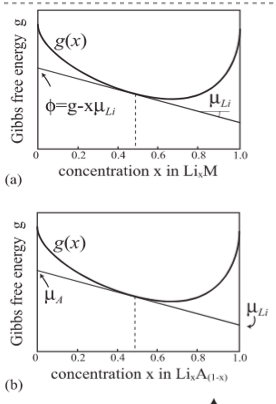
\includegraphics[scale=2]{figures/thermodynamics_vanderven.png}
    \caption{Representation of the connection between the Gibbs free energy, $G(x)$, the  lithium chemical potential $\mu(x)$ in (a) an intercalation electrode and (b) an alloy electrode. Reproduced from \cite{VanderVen2020}}
    \label{fig:vanderven_thermodynamics}
\end{figure}

In the case of a lithium ion cell the equilibrium cell voltage, $\phi(x)$, and the chemical potential of intercalated Li, $\mu(x)$, are related as:

\begin{equation}
    \phi(x) = -\frac{\mu(x) - \mu_{\rm{Li}}^{\rm{ref}}}{nF},
    \label{eq:potchempot_raw}
\end{equation}

where $\mu_{\rm{Li}}^{\rm{ref}}$ is the chemical potential of the reference electrode, $n$ is the number of electrons transferred per formula unit of intercalation host ($n =1$ for Li-ion cells), and $F$ is the Faraday constant. The most convenient reference potential, both from the point of view of simulations and for comparison with experimental measurements of Li-ion half cells, is the bcc metallic Li anode. With a suitable choice of units for all potentials ($\mu$ expressed in eV per formula unit of intercalation host), equation~\ref{eq:potchempot_raw} can be written much more simply as: \cite{CEDER1999131}

\begin{equation}
    \phi(x) = -\mu(x).
    \label{eq:potchempot}
\end{equation}

The intercalated Li chemical potential is defined by:

\begin{equation}
    \mu(x) = \left(\frac{\partial{\underline{G}(x)}}{\partial{N_{Li}}}\right)_{p,T,N_{\rm{host}}} = \left(\frac{\partial{G(x)}}{\partial{x}}\right)_{p,T,N_{\rm{host}}},
    \label{eq:chemicalpotgibbs}
\end{equation}

where $\underline{G} =$ the absolute (i.e. extensive) Gibbs free energy of Li dissolution into the host, $p =$ pressure, $T =$ the absolute temperature, and $N_{\rm{host}}$ and $N_{\rm{Li}}$ are respectively the number of host and lithium atoms in the system. The subscripts $p$, $T$, and $N_{\rm{host}}$ will be implicitly assumed constant from now on and dropped to simplify notation.

Similarly it is well known that:

\begin{equation}
    \frac{\partial{G(x)}}{\partial{x}} = \frac{\partial{H(x)}}{\partial{x}} - T\frac{\partial{S(x)}}{\partial{x}}, 
    \label{eq:gibbshs}
\end{equation}

where $H(x)$ and $S(x)$ are the enthalpy and entropy, respectively, per formula unit of host material.

We can use equations \ref{eq:potchempot}, \ref{eq:chemicalpotgibbs}, and \ref{eq:gibbshs} to get $\partial{G}/\partial{x} = -E_{\rm{OCV}}$, then, taking the derivative of the OCV with respect to $T$ and using the chain rule, we obtain:

\begin{equation}
   \frac{\partial{S(x)}}{\partial{x}} = \frac{\partial{E_{\rm{OCV}}(x)}}{\partial{T}}
    \label{eq:entropy_measurement}
\end{equation}
and so,
\begin{equation}
    \frac{\partial{H(x)}}{\partial{x}} = T\frac{\partial{E_{\rm{OCV}}(x)}}{\partial{T}} - E_{\rm{OCV}}(x).
    \label{eq:enthalpy_measurement}
\end{equation}

Due to the units of eV per formula unit for the potentials $H(x)$ and $TS(x)$, i.e. as in the conversion between equations~\ref{eq:potchempot_raw} and \ref{eq:potchempot}, the usual factors of $F$ have been omitted. In this way it is possible to simulate not only the equilibrium voltage, but split its contributions into enthalpy and entropy components. Both components can be experimentally measured \cite{schlueter_quantifying_2018,Mercer2019,THOMAS2003844,Reynier2004,Yazami_2006} and modelled through Monte Carlo or mean field methods \cite{schlueter_quantifying_2018,mercer_influence_2017,Mercer2019,Leiva2017b}, providing additional properties for model validation purposes and to check the temperature dependence of those properties is modelled accurately. A good thermodynamic basis can then be used to derive dynamic properties as outlined in the subsequent sections.

\subsubsection{Activity coefficients of electrolytes (Arihant)}
\label{sec:tf}

The activity coefficient of electrolytes can be computed from DFT+\pbe{} models described in section \ref{sec:dft+cont}.\cite{Ringe2016, Dziedzic2020} The notation used here follows from that section. The activity coefficients of electrolytes ($\gamma_j$, $j=1\dots p$) describe the behaviour of non-ideal electrolytes, and the dependence of their chemical potentials on electrolyte concentration $\{\ci\}$.\cite{Atkins2014}

\begin{equation}
    \label{eq:mujid}
    \mu_j\left[\{\cif\}\right]=\mu_j\left[\{\cif=0\}\right]+ \kb T\ln{\gamma_j},  \ j=1\dots p
\end{equation}

The chemical potential of the quantum solute represents the change in the free energy per number of molecules ($n_j$, $j=1\dots p$) of solute:

\begin{equation}
    \label{eq:dtdn}
    \frac{\partial \Omega}{\partial n_j}\bigg|_{\{\cif\}}=\frac{\partial \Omega}{\partial n_j}\bigg|_{\{\cif=0\}}+ \kb T\ln{\gamma_j}, \ j=1\dots p
\end{equation}

This can be written in terms of solvation energies as the energies of solute $j$ in vacuum cancel out:

\begin{equation}
    \label{eq:dtc}
    \Delta\Omega_j\left[{\{\cif\}}\right]-\Delta\Omega_j\left[{\{\cif=0\}}\right]=\kb T \ln{\gamma_j}, \ j=1\dots p
\end{equation}

or, equivalently

\begin{equation}
    \label{eq:activityj}
    \frac{\Delta\Delta\Omega_j\left[\{\cif\}\right]}{\kb T} =\ln{\gamma_j}, \ j=1\dots p.
\end{equation}

Hence, activity coefficients can be computed from the electrolyte effect on solvation energies ($\Delta\Delta\Omega$), as described in section \ref{sec:dft+cont}. The mean activity coefficient of all the $p$ electrolytes species can be calculated as:
\begin{equation}
    \label{eq:activitymean}
    \ln \gamma_{\rm mean} = \frac{1}{p}\sum_{j=1}^p \ln \gamma_j.
\end{equation}

\subsubsection{Diffusion coefficients (Lucy/Maxim)}
\label{sec:diffusion}

The \textit{diffusion coefficient} is a term used to describe the rate of ion transport within a system. This term, however, has been used in literature to express several forms of diffusion, which characterise diffusion in a material in different ways. Here, we describe several commonly used forms of \textit{diffusion coefficient}, in context of where they are used, focused on bulk diffusion. A detailed description of diffusion along grain boundaries and along surfaces is given in reference \citenum{heitjans2006diffusion}, Chapters 7 and 8.

Ionic transport within the electrodes and electrolyte plays a vital role in the kinetics of a battery. It can fundamentally be described with flux expressions that relate ion fluxes to chemical or electrochemical potential gradients. This is related by Fick's first law, where the diffusion flux, $\boldsymbol{\jmath}$, is described using the gradient of the concentration, $c$, via:

\begin{equation}
    \boldsymbol{\jmath} = - \mathcal{D} \nabla c
    \label{eq:fickfirst}
\end{equation}

$\mathcal{D}$ is denoted as the diffusion coefficient tensor or diffusivity tensor, and implies that $\mathcal{D}$ varies with direction. In general, the diffusion flux and concentration gradient are not always antiparallel. They are antiparallel for isotropic mediums. This is discussed in more detail in reference \citenum{heitjans2006diffusion}.

Steady state methods for measuring diffusion coefficients, like the permeation method, \cite{heumann2013diffusion} are directly based on Fick's first law. In a non-steady states, the diffusion flux and concentration vary with time, $t$, and position $x$, and a balanced equation is necessary. For particles which undergo no reaction this become the continuity equation:

\begin{equation}
    \frac{\partial c}{\partial t} + \nabla {\boldsymbol{\jmath}} = 0
    \label{eq:continuity}
\end{equation}

Combining equations \ref{eq:fickfirst} and \ref{eq:continuity} leads to Fick's second law, also called the diffusion equation, which predicts how diffusion causes the concentration to change with time:

\begin{equation}
    \label{eq:ficksecond}
    \frac{\partial c}{\partial t} = \nabla (\mathcal{D} \nabla c )
\end{equation}

In diffusion studies with trace elements the material composition does not practically change and $\mathcal{D}$ is independent of the tracer concentration, presenting a concentration-independent diffusion coefficient. For diffusion in multiple dimensions Fick's second law becomes: \cite{crank1979mathematics}

\begin{equation}
    \frac{\partial c}{\partial t} = \mathcal{D} \nabla^2 c
    \label{eq:nodirectional_diffusion}
\end{equation}

The temperature dependence of the diffusion coefficient is often described empirically by an Arrhenius relation:

\begin{equation}
    \mathcal{D} = \mathcal{D}_0 \cdot \textrm{exp} \left (- \frac{E_A}{k_B T} \right )
\end{equation}

where $E_A$ is the activation energy for the mass transport, $D_0^T$ is the pre-exponential factor, $k_B$ is the Boltzmann constant, and $T$ is the temperature.

From the microscopic point of view, the tracer diffusion coefficient can be defined by the Einstein-Smoluchowski relation, \cite{einstein1905presumed,von1906kinetischen}

\begin{equation}
    \mathcal{D} = \lim_{t\to\infty} \frac{\left <r^2(t)\right >}{2dt}, \mathrm{where} \left <r^2(t)\right > = \left< \left(x(t) - x_0 \right)^2 \right>
    \label{eq:self-diffision}
\end{equation}

Here, $\left <r^2(t)\right >$ is the mean square displacement (MSD) of the particles after time $t$ and $d$ is the dimensionality of the movement. This is also known as the \textit{self diffusion coefficient} and is the main approach used to calculate the diffusion coefficient in kinetic Monte Carlo (kMC) and Molecular Dynamics (MD) from the atom trajectories. This is discussed in more detail in reference \citenum{VanderVen2020}.

In atomistic modelling, diffusion coefficients can also be calculated using other approaches, such as Green-Kubo. The Green-Kubo approach is linked to the Einstein-Smoluchowski relation approach. Both approaches assumes that particle dynamics can be well approximated by a Brownian motion. As described in equation~\ref{eq:self-diffision}, Brownian motion of independent particles can be expressed by the MSD of a particle proportional to time. This can also be termed as the integral of the velocity. The Green-Kubo approach is derived from the integration of the velocity (or current) autocorrelation function. Assuming that dynamics is ergodic, the diffusion coefficient can be calculated using a linear fit to the velocity autocorrelation function. Averaging is applied to this, for example, a time  average for a selected particle type, a sample average, or an ensemble average.

% This relates to linear response through:

% \begin{equation}
% x(t) - x(0) = \displaystyle\int_0^t u (\tau) d \tau ,
% \end{equation}

% after some rearranging, this can be expressed as:

% \begin{equation}
% D = \displaystyle  \lim_{t\rightarrow \infty} \frac{1}{t d} \int_0^t d \tau_1 \int_0^{t-\tau_1}d\tau_2 \langle u(\tau_1) u (\tau_1 + \tau_2) \rangle
% \label{velAC}
% \end{equation}

% Where, $t$ is time, $d$ is ???, $u$ is ???, and  $\tau$ is ????????.

% % {\color{red} \tiny Clarify: averaging method and meaning of the limit, see comments above Eq. (83)-- MZ} 

% There are several approaches to how transport parameters are modelled in MD simulations, outside of using the trajectories as described above, which use different physics ideas. These approaches have to resolve difficult issues like the nature of irreversibly, the right implementation of statistical ensemble or averaging method, and cutoffs of singular potentials. A comprehensive discussion regarding these would be an in-depth review in itself, and therefore is outside the scope of this review. Here, we briefly review two widely used approaches, Green-Kubo and Linear response, with a method based on the Stefan-Maxwell-Onsager discussed in section~\ref{sec:stefan-maxwell}. These approaches are discussed in terms of extracting diffusion coefficients which are comparative to those used in continuum models, in aid for parameterisation use.

% It is generally accepted that continuum electrochemical transport equations, both in electrodes and electrolytes, are of diffusion type, which are unlike the Newtonian dynamics equations that are dissipative and time-irreversible. Molecular dynamics simulations can be used to determine parameters of continuum models from details of microscopic forces between particles. To be comparative to continuum theory, the relationship between the fluxes of the appropriate macroscopic quantities and their values and the gradients, such as species concentrations, temperature, and pressure, needs to be determined.

% In addition, there is a fundamental difficulty since the dynamics of finite particle systems is time-reversible, while the continuum dynamics it aims to describe is not. Thus a good choice of thermostat is required in molecular dynamics simulations for any chance to reconcile the atomistic and continuum approaches. On the one hand MD provides dissipation, but on the other, does not provide artifacts altering underlying microscopic physics.

% {\bf Green-Kubo.}
% The Green-Kubo approach tacitly assumes that, in a certain statistical sense, particle dynamics can be well approximated by a Brownian motion. This is well understood and has solid mathematical footing, due to works of Ito, Stratonovich, and others.

% As described in equation~\ref{eq:self-diffision}, Brownian motion of independent particles can be expressed by the mean square displacement of a particle proportional to time. This relates to linear response through:

% \begin{equation}
%     x(t) - x(0) = \displaystyle\int_0^t u (\tau) d \tau ,
% \end{equation}

% after some rearranging, this can be expressed as:

% \begin{equation}
%     D = \displaystyle  \lim_{t\rightarrow \infty} \frac{1}{t d} \int_0^t d \tau_1 \int_0^{t-\tau_1}d\tau_2 \langle u(\tau_1) u (\tau_1 + \tau_2) \rangle
% \end{equation}

% In the context of MD, and assuming that dynamics is ergodic, this suggests that the diffusion coefficient can be modeled by a linear fit to the displacement autocorrelation function, with averaging applied. This averaging can be, for example, a time series average for a selected marker particle, a sample average, or an ensamble average, where the initial configurations sampled in the phase space with weights added in accordance with a given probability distribution.

% % ({\bf select: multiple choice}):

% % {\scriptsize \color{red}\noindent  Equations below will go away but method of averaging needs to be stated in words. equations are for clarification of the issue.}

% % {\scriptsize   \color{red} \noindent Since in MD computational box is bounded, so is $(x(t) - x(0))^2$ in eq. 80; therefore, the limit in (80) , taken it literally, =0. For that reason, it needs to be interpreted as the best linear fit, not as the stated limit. MZ}

% % \noindent time series average for a selected marker particle,

% % \begin{equation}
% %     \mbox{acx}_1(t) \approx \displaystyle \sum_{i=1}^{N} \frac{1}{2   d N} \langle ( \, \mathbf{x}(t+ \tau_i) - \mathbf{x}(\tau_i) ) \,^2 \rangle   {\stackrel{\mbox{\tiny linear fit}}{\approx}}  D t + C
% % \end{equation}

% % or sample average,

% % \begin{equation}
% %     \mbox{acx}_{\mbox{\tiny N}}(t) \approx \displaystyle \sum_{i=1}^{N} \frac{1}{2 d N} \langle ( \, \mathbf{x}_i(t) - \mathbf{x}_i(0) ) \,^2 \rangle   {\stackrel{\mbox{\tiny linear fit}}{\approx}}  D t + C
% % \end{equation}

% % or ensemble  average, with initial configurations sampled in the phase space with weights $\lambda_i$, drawn according to some probability distribution, say Gibbs

% % \begin{equation} \begin{array}{l}
% %     \mbox{acx}_e(t) \approx \displaystyle \frac{1}{Z} \sum_{i=1}^{N}  \frac{\lambda_i}{2 d}  \langle ( \, \mathbf{x}_i(t) - \mathbf{x}_i(0) ) \,^2 \rangle   {\stackrel{\mbox{\tiny linear fit}}{\approx}}  D t + C ,
% %      \\
% %      \displaystyle \sum_{i=1}^{N} \lambda_i =Z.
% % \end{array} \end{equation}

% {\bf Linear response.}
% Linear response methods are more widely used compared to the Green-Kubo methods, however, they involve assumptions such as Brownian motion or a prescription of dissipative function, and seem to provide no guarantee apriory that diffusion coefficients computed that way will accurately reproduce required macroscopic fluxes. It is understood, since the work of \citeauthor{einstein1905presumed} and \cite{von1906kinetischen}, \cite{einstein1905presumed,von1906kinetischen} that there is a relation between diffusion coefficient and mobility, balancing diffusion and drift as:

% \begin{equation}
%     D = \mu k_b  T
% \end{equation}

% The diffusion coefficient can therefore be computed through calculating the response of an equilibrium system to applied generalised force. In the Newman's continuum modeling framework of concentrated solution theory, the driving force is the gradient of the chemical potential. This is not easy to implement, but kinetic theory of gases suggests that response to the gradient of the chemical potential, or to a force, is the same.

% The linear response theory, is described in detail in  references ~\citenum{GrootMazur} and \citenum{Ruelle_2009}. Its use in continuum concentrated solution theory, an important part of electric battery models, is described in references \citenum{2002PhDWheeler} and \citenum{Wheeler2004_1}. Here we give a brief outline following \citeauthor{MorissEvans1987}'s description. \cite{MorissEvans1987} 

% Let $B (\Gamma)$, where $\Gamma = (p,q)$, be a function of interest on the phase space, where $p$ are particle momenta and $q$ are coordinates. Time dependence of $B$ is determined by particle dynamics, $ B(t) = B (\Gamma (t, \Gamma_0))$, where $\Gamma (t, \Gamma_0))$ is the dynamical flow, with initial conditions $\Gamma_0$. $f(\Gamma_0)$ is a probability distribution on the phase space, which is invariant under unperturbed flow. Statistical averaged quantities are computed as:

% \begin{equation}
%     \langle B(t) \rangle = \displaystyle\int B(\Gamma (t, \Gamma_0)) f(\Gamma_0) d\Gamma_0 
%     %:= \displaystyle\int B(0) f(\Gamma,t) d\Gamma
% \end{equation}

% Which, when integrated by parts becomes: 

% \begin{equation}
%     \frac{d}{dt} \langle B(t) \rangle = \displaystyle\int \dot{\Gamma}\frac{\partial B(t) }{\partial \Gamma} f (\Gamma_0) d\Gamma_0 = - \displaystyle\int   B(t) \frac{\partial  }{\partial \Gamma} ( \, \dot{\Gamma} f (\Gamma_0)) \,  d\Gamma_0
% \end{equation}

% In the unperturbed case, according to Liouville theorem and the invariance of $f$ under the flow, $f(\Gamma_0) d\Gamma_0 = f(\Gamma) d\Gamma$. If $f$ is a Gibbs distribution, $f_0$, with Hamiltonian, $H_0,$, then $\frac{\partial  }{\partial \Gamma} ( \, \dot{\Gamma} f_0 (\Gamma)) \, =   \dot{\Gamma} \frac{\partial  }{\partial \Gamma}    f_0 (\Gamma) = -\beta \dot{H_0} f_0 (\Gamma)$. In the unperturbed case, $\dot{H_0} =0$ and $\langle B(t)\rangle$ are time independent. In the perturbed case: 

% \begin{equation}
%     \dot{H_0} = V J F, 
% \end{equation}

% where $F$ is generalised force, $J$ is generalised flux, and $V$ is the volume. In the first order in perturbation: 

% \begin{equation} \begin{array}{l}
%      \frac{d}{dt} \langle B(t) \rangle = \displaystyle\int \dot{\Gamma}\frac{\partial B(t) }{\partial \Gamma} f (\Gamma_0) d\Gamma_0 = \beta V F  \displaystyle\int   B(t) J(0) f (\Gamma_0)) \,  d\Gamma_0 = \beta V F  \langle B(t) J(0) \rangle;
%      \\
%     \langle B(t) \rangle =   \langle B(0) \rangle +  \beta V F  \displaystyle \int_0^t \langle B(t) J(0) \rangle
% \end{array} \end{equation}

% Applying this to the current statistical average and assuming that in the unperturbed case current average is zero, we get:

% \begin{equation}
%     \langle J(t) \rangle =  \beta V F \displaystyle\int_0^t \langle J(s) J(0) \rangle ds .
% \end{equation}

% Linear response is understood as response, per unit of generalised force, as $t\rightarrow \infty,$ such as: 

% \begin{equation}
%     L =   \beta V \displaystyle\int_0^{\infty} \langle J(s) J(0) \rangle ds.
% \end{equation}

% The above considerations in particular apply to compute averaged flux $n \mathbf{v}$ in response to applying force. Such flux, per single particle, is particle mobility, which relates to diffusion coefficient by the Einstein relation described in equation~\ref{eq:self-diffision}. 

% \textbf{Creating a flow by creating concentrations gradients}. This would be the most intuitive way to test Fick's law and determine diffusion coefficients. However, multi-species flows may be very complicated, for example not uniform, creating difficulties in this approach.This is discussed in greater detail in Refs.~\citenum{2002PhDWheeler} and \citenum{Wheeler2004}.

\subsubsection{Vibrational and Thermal Properties (Hui)}
\label{sec:thermal_electronic_vibrational}

While molecular dynamics simulates the evolution of a chemical system over time, lattice dynamics is an approach that models the underlying vibrations. In crystalline solids, extended vibrations can be described as phonons with a characteristic frequency and wavevector, $\omega(q)$. A unit cell with $N$ atoms contains 3$N$ phonon modes. The theory of phonons provides a direct connection between microscopic atomic motion and macroscopic properties including specific heat capacity, IR and Raman spectra, and thermal expansion.\cite{ladd1986lattice, turney2009predicting,seko2015prediction} 

While assuming that phonons are harmonic simplifies the theoretical description, it is necessary to include anharmonic effects to describe phenomena such as heat transport. The lattice thermal conductivity, $\kappa$, depends on the lifetime of each phonon, i.e. how long it persists before decaying, which is an anharmonic process. Formally, the thermal conductivity given by the product of the modal heat capacity, ($C_V$), the group velocity, $v$, and the phonon mean free path, $v \times \tau$ (where $\tau$ is the phonon lifetime). The macroscopic $\kappa$ is obtained by summing over band indices, $v$, averaging over wavevectors, $q$, and normalising by the unit cell volume:

\begin{equation}
    \kappa = \frac{1}{NV_0} \,\sum_{qv} C_{V,qv} v_{qv} \otimes v_{qv} \tau_{qv}
    \label{eq:thermal}
\end{equation}

where $N$ is the number of unit cells in the crystal (number of wavevectors in the Brillouin zone summation) and $V_0$ is the volume of the crystallographic unit cell.

The heat capacity and group velocity can be extracted from the harmonic phonons, which are readily accessible from calculations based on first-principles or classical potential methods. The lifetime of each phonon mode is more demanding to compute and is often performed within a many-body perturbation theory expansion of phonon-phonon interactions. One approximation is to consider only the leading term of three-phonon creation and annihilation. \cite{togo_distributions_2015} However, higher-order processes may limit the lifetimes, depending on the material and temperature. There are a range of packages available to compute the terms in Eqn. \ref{eq:thermal} including \textsc{Phono3py} \cite{phono3py} (recently applied to \ce{LiCoO2} and NMC cathodes)\cite{yang2019highly,yang2020chemical}, \textsc{ALAMODE}\cite{tadano2014anharmonic}, and \textsc{ShengBTE}\cite{ShengBTE_2014}.

 \end{document}